\documentclass[12pt,a4paper]{article} % Defines the document as an article with 12pt font on A4 paper
\usepackage[utf8]{inputenc} % Sets UTF-8 encoding
\usepackage{geometry} % Enables page geometry customization
\geometry{margin=1in} % Sets 1-inch margins
\usepackage{graphicx} % Allows inclusion of images
\usepackage{titlesec} % Controls section formatting
\usepackage{hyperref} % Enables hyperlinks
\usepackage{tikz}
\usepackage{float}
\usepackage{amsmath}
\usetikzlibrary{shapes.geometric, calc, arrows.meta, positioning}
\usepackage{setspace} % Allows line spacing adjustments
\usepackage{csquotes} % Improves quotation handling
\usepackage{datetime} % Provides date and time formatting
\usepackage{enumitem}
\usepackage[backend=biber,style=apa, sorting=nyt]{biblatex} % Configures bibliography using Biber with APA style
\addbibresource{references.bib} % Adds a bibliography file (replace with your .bib file name)
\renewcommand{\dateseparator}{-} % Sets date separator as '-'
\onehalfspacing % Sets line spacing to 1.5


\title{\textbf{Research Proposal: PhD candidate in Industrial Engineering}} % Defines the title
\author{
	\textbf{Benjamin R. Berton}\\
	Polytechnique Montréal\\
	\href{mailto:benjamin.berton@polymtl.ca}{benjamin.berton@polymtl.ca}\\
	\textit{Supervised by: Philippe Doyon-Poulin}
} % Defines author details

\begin{document} % Begins the document
	\maketitle % Generates the title
	
	\begin{center}
		\textbf{A cognitive modelling approach to evaluating Human-Autonomy Teaming in commercial aviation}
	\end{center} % Centers the research title
	
	\begin{center}
		Submitted to members of the Jury:\\
		Pr. Jean-Marc Frayret, Pr. Philippe Doyon-Poulin \& Pr. Shi Cao\\
		\date{\today} % Inserts today's date
	\end{center} % Centers the research title
	
	\newpage % Starts a new page
	
	\tableofcontents % Generates the table of contents
	\newpage % Starts a new page
	
	\section{Trigger \textbf{TBD}} % Defines a section titled "Trigger"
	Commercial aviation has shown a trend toward crew reduction, progressively decreasing the number of members in the cockpit \parencite{harris_human-centred_2007}. Historically, flight crews included up to five members, but technological advancements have reduced this number to two—the Captain (CPT) and First Officer (FO)—eliminating the need for flight engineers, navigators, and radio operators.
	
	Currently, the Federal Aviation Administration (FAA) - Part 25 regulations mandate a minimum of two pilots in the cockpit. However, technological advancements suggest the possibility of transitioning to Single Pilot Operations (SPO), where only one pilot would be on duty, assisted by advanced onboard technologies and potentially ground support \parencite{bilimoria_conceptual_2014}. While this transition is technically feasible, it introduces significant challenges, far more complex than previous crew reductions \parencite{matessa_using_2017}.
	
	One of the main issues with SPO is the removal of a redundancy layer, a fundamental element of aviation safety. Shifting from a two-pilot cockpit to a single-operator model requires ensuring an equivalent or higher level of safety compared to current operations \parencite{boy_requirements_2014}. Simply replacing the human co-pilot with increased automation is not a viable solution. Future operational concepts must rethink task distribution between the pilot and autonomy to maintain reliability and resilience.
	
	Successfully integrating SPO into commercial aviation requires moving beyond the traditional Human-Centered Design (HCD) approach. It is crucial to adopt a Human Systems Integration (HSI) perspective to ensure a seamless consideration of technical, organizational, and human dimensions throughout the system's lifecycle \parencite{boy_prodec_2024}. This transition will involve structural changes within air traffic management, raising new safety concerns. Identifying design flaws, anticipating potential human errors, and addressing them early in the development process are essential. The HSI approach allows for these aspects to be considered within a global operational framework, integrating interactions between human and technological elements.
	
	Another key factor for the success of SPO is the collaborative aspect between humans and advanced automated systems, known as Human-Autonomy Teaming (HAT). This approach emphasizes effective cooperation between the single pilot and advanced autonomous systems, where these systems do more than assist—they act as teammates \parencite{shively_autonomy_2017}.
	
	HAT is based on the evolution from automation to autonomy. Automation refers to technologies that process data, make decisions, and execute tasks based on predefined procedures \parencite{hoff_trust_2015, hancock_imposing_2017}. Autonomy, on the other hand, refers to a system's ability to perform tasks with minimal human intervention over an extended period \parencite{endsley_here_2017, holbrook_enabling_2020}. This progressive shift toward greater autonomy fundamentally changes the human-automation relationship, evolving from simple interaction to genuine teamwork \parencite{endsley_here_2017}.
	
	However, increasing automation levels also presents challenges, particularly automation complacency, where excessive reliance on automated systems can lead to reduced vigilance and an inability to react effectively in case of anomalies \parencite{lee_design_2023}. To avoid this pitfall, it is crucial to design systems that promote active collaboration between the pilot and onboard autonomy \parencite{endsley_here_2017}. The goal of HAT is to ensure smooth and efficient cooperation, where autonomous systems act as real teammates, contributing to safer and more effective flight operations \parencite{mcneese_chapter_2020}.
	
	\section{Theoretical Background \textbf{TBD}}
	\subsection{Human-Autonomy Teaming}
	\subsection{Situation Awareness}
	\subsubsection{Team-Situation Awareness}
	\subsubsection{Computational models of Situation Awareness}
	\subsection{Knowledge gap} % Section title "Knowledge Boundaries"
	
	%\section{Research Question and Hypothesis} % Section for research question and hypothesis
	%\textbf{Question:} How does introducing a virtual co-pilot based on a cognitive model influence pilot performance and situation %awareness in Single Pilot Operations?
	%
	%\textbf{Hypothesis:} A virtual co-pilot, designed with a rigorous cognitive model, improves pilot situation awareness while %reducing cognitive load.
	
	\section{Objectives} % Defines the "Objectives" section
	The general objective of this research is to develop a methodology that facilitates the design of an autonomous agent collaborating with a human pilot for commercial aviation operations. To do so, we will use a collection of methods from the human factors and ergonomics research domain, design an agent, and investigate how the design of the human-autonomy teamwork and agent interface impacts the Team Situation Awareness.
	
	To achieve this objective, the thesis will be comprised of three phases.
	\begin{enumerate}[label=\textbf{\arabic*.}]
		\item We will conduct a thorough analysis of the work and design domain in order to delineate the taskwork and teamwork and list requirements for the agent design. Especially:
		\begin{enumerate}[label=\textbf{\arabic{enumi}.\Alph*.}]
			\item \label{obj:1a} Identify the goal hierarchy that pilots use to achieve high levels of safety and performance in current day operations.
			\item \label{obj:1b} List the information required to construct a good Situation Awareness 
		\end{enumerate}
		\item We will develop in parallel a cognitive model of the human pilot and the autonomous agent, enabling them to interact in a closed-loop simulation environment. 
		\begin{enumerate}[label=\textbf{\arabic{enumi}.\Alph*.}]
			\item \label{obj:2a} Combine QN, ACT-R, and SEEV theory to create a cognitively plausible model of human pilot's perception of elements in the current situation (level 1 Situation Awareness)
			\item \label{obj:2b} Model the task using outputs from the GDTA and IA so that the cognitive model is capable of navigating the scenario on its own.
			\item \label{obj:2c} Develop an agent that can perform the tasks described in the IA.
			\item \label{obj:2d} Develop an Human-Agent Interface that comply with the teaming requirements established in the IA and modify the cognitive model so that it now has to team with the autonomy to navigate the scenario.
		\end{enumerate}  
		\item We will conduct Human-In-The-Loop Simulation studies with expert pilots in order to :
		\begin{enumerate}[label=\textbf{\arabic{enumi}.\Alph*.}]
			\item \label{obj:3a} Validate the cognitive model
			\item \label{obj:3b} Investigates the human factors that weren't modeled such as trust in the autonomous agent and usability of the interface.
		\end{enumerate}
	\end{enumerate}
	These phases will be detailed in the next section 

	
	\section{Methodology} % Section title "Methodology"
	\subsection{The use-case scenario}
	The preliminary step for applying the methodology is to select a proper use case scenario, that is (1) realistic, so that information is easily available for modelling and knowledge gained can benefit the aviation industry, (2) challenging enough so that teaming with an autonomous agent is strongly beneficial for achieving good performance, and (3) procedural, deterministic, and short enough so that the cognitive modelling and agent implementation can realistically be implemented inside Polytechnique's flight simulator platform.
	
	The scenario consists in a takeoff and initial climb phase with an engine failure due to a bird or drone strike. The scenario is performed by a single pilot in a multi-engine very light jet aircraft. Take-off with an engine failure is a challenging scenario for single pilot operations that is highly dynamic and require fast and precise decision-making from the captain. Bird and drone strike will be an issue for the foreseeable future of commercial aviation and is therefore a scenario of particular interest for the industry.

	\begin{figure}[H]
 		\centering
  		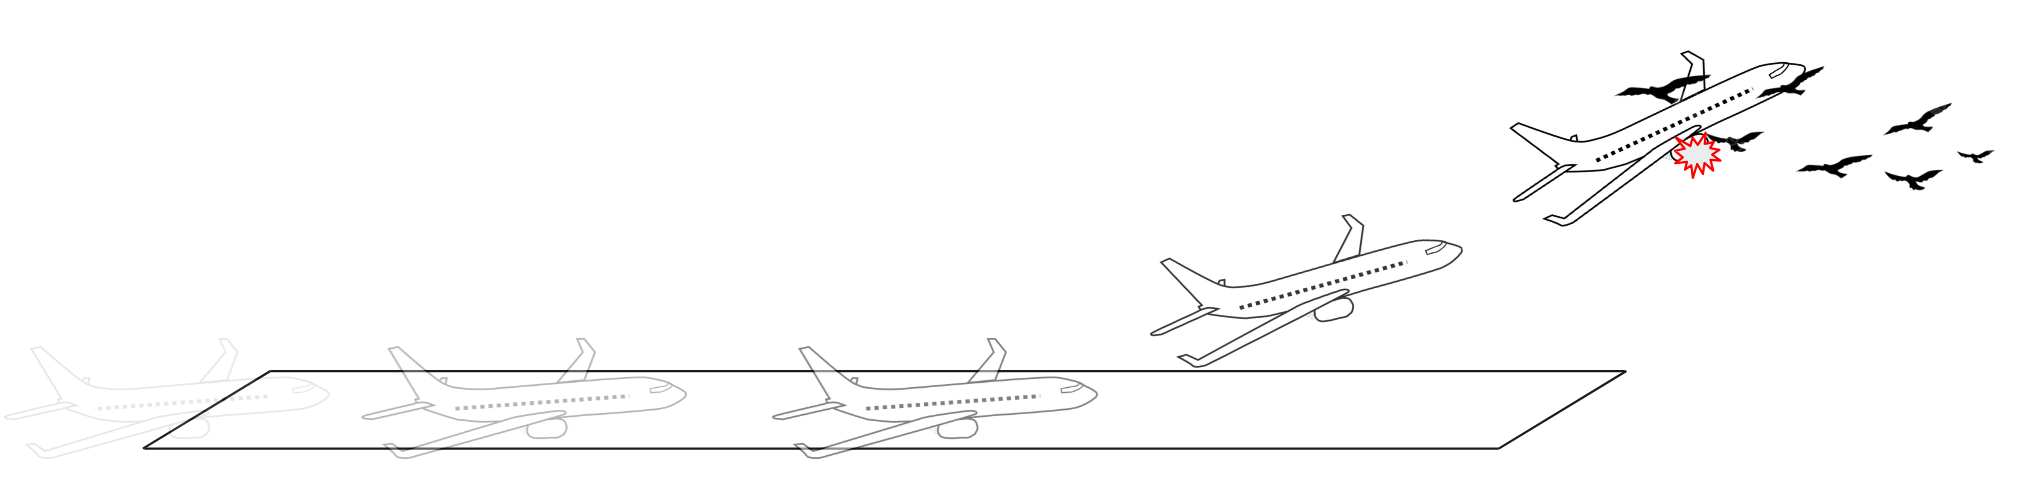
\includegraphics[width=1\textwidth]{./images/scenario.png}
   		\caption{Takeoff scenario with a birdstrike causing an engine failure.}
		\label{fig:takeoff-scenario-simplified}
	\end{figure}

	\subsection{Phase 1: Work and design domain analysis}
	The first step of the methodology involves analyzing the current state of commercial aviation operations to understand the scope of the to-be-designed Autonomous Agent (AA). Two complementary methods are used, the Goal Directed Task Analysis (GDTA) and the Interdependence Analysis (IA).

	\subsubsection{Goal-Directed Task Analysis}
	A GDTA was conducted to understand the information needs inherent to commercial aviation operations. GDTA is a task analysis methodology aimed at identifying the critical information human operators must acquire and process to achieve their mission goals effectively and safely. This information contributes to the construction and maintenance of Situation Awareness (SA), a key predictor of operational performance and safety in commercial aviation \parencite{endsley_here_2017}. %Verify this ref, goal is to say SA is predictor of operational performance. SotA on SA might be good
	Following the established GDTA outlined by Endsley and Jones for a complete commercial aviation flight \parencite{endsley_designing_2003}, our GDTA was constructed by selecting the relevant hierarchy of goals and associated information requirements for our takeoff scenario. To enrich and validate the GDTA, four experienced commercial pilots were recruited and interviewed. Their insights were incorporated to ensure that the analysis reflects the operational realities of contemporary flight environments.

	The GDTA resulted in a hierarchically organized representation of pilot goals see Figure~\ref{fig:goal-hierarchy}, each associated with the specific information necessary for optimal task performance see Figure . This structured output serves as a foundation for designing the human-autonomy team. Specifically, the identified information elements will guide the development of the Autonomous Agent, ensuring that both the human pilot and the synthetic teammate maintain a sufficient level of SA throughout the operation (the complete results of the GDTA can be found in Appendix~\ref{appendix:GDTA}).


	\begin{figure}[H]
		\centering
		\begin{minipage}[b]{1\textwidth}
			\centering
			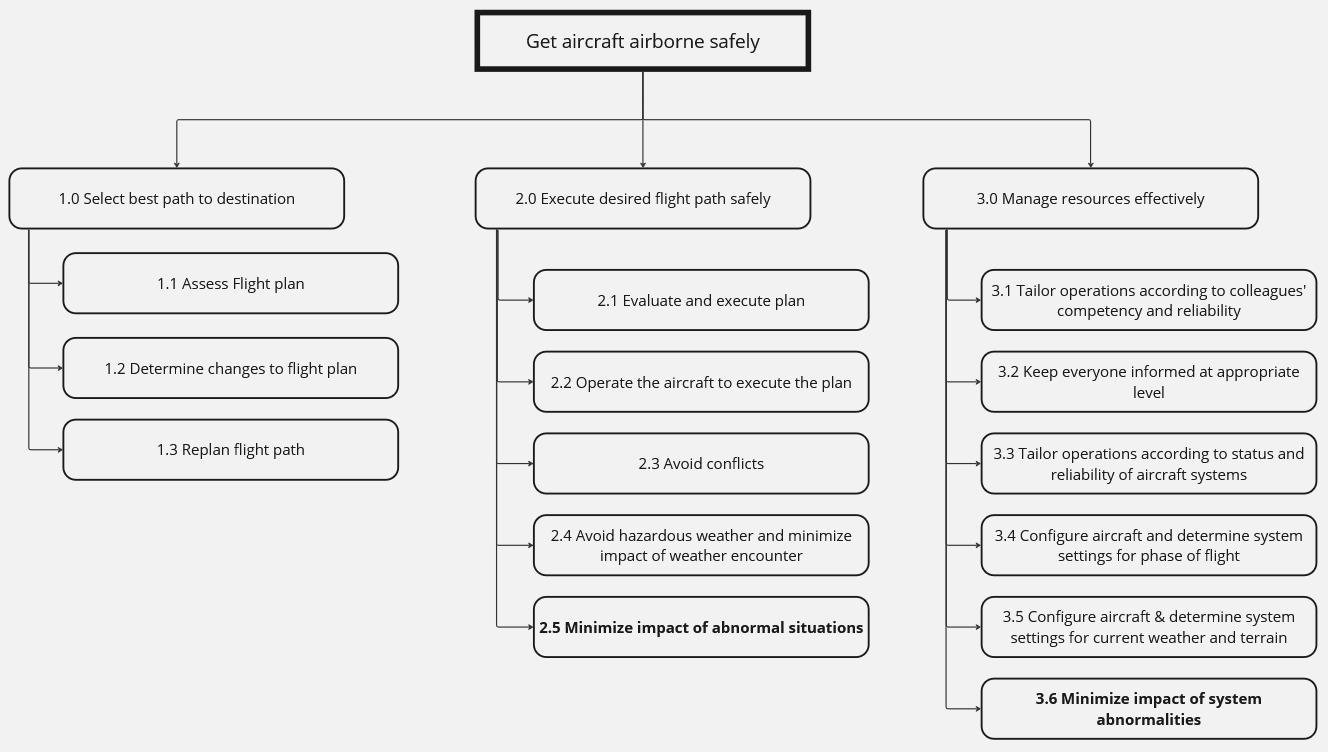
\includegraphics[width=1\textwidth]{./images/gdta_goal_hierarchy.jpg}
			\caption{High-level goal hierarchy}
			\label{fig:goal-hierarchy}
		\end{minipage}
		\begin{minipage}[b]{1\textwidth}
			\centering
			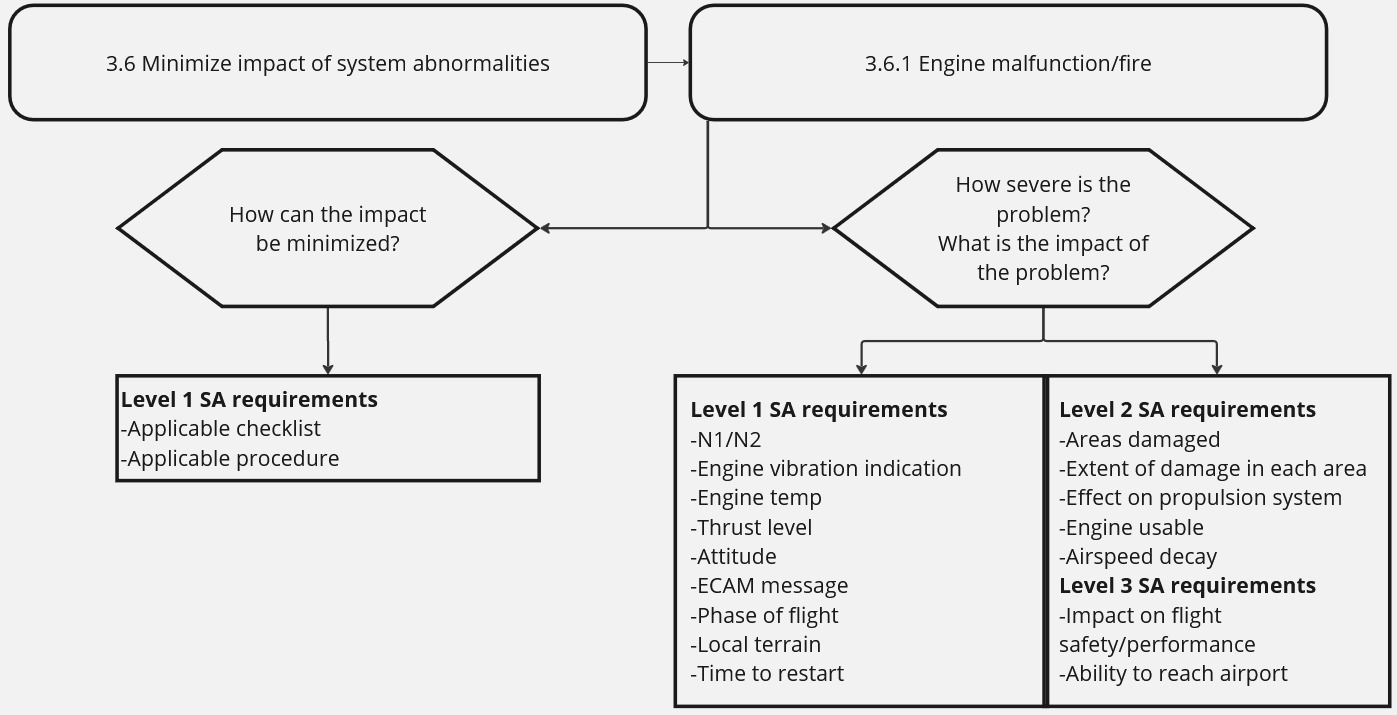
\includegraphics[width=1\textwidth]{images/goal_and_info_req.jpg}
			\caption{Information requirements for goal \textit{3.6.1 - Engine malfunction/fire}}
			\label{fig:info_req}
		\end{minipage}
	\end{figure}

	The goal is to ensure that the closely coupled human-agent team maintains alignment of their respective situation representation by attending both to the proper information for the task at hand (see for example Figure~\ref{fig:info_req}). This alignment supports the development of Team Situation Awareness (Team SA)—the state in which each teammate possesses an accurate understanding of the situation relevant to their roles within the flight deck.
	This notion is visually represented by Figure~\ref{fig:team-sa-venn}, where individual SA of each team member contributes to the larger construct of Team SA. Furthermore, a significant overlap in individual SA defines the concept of Shared Situation Awareness. Achieving and maintaining both individual SA and shared SA between the human and autonomous teammate is critical to ensuring coordinated, safe, and effective operations.

	\begin{figure}[h!]
		\centering
		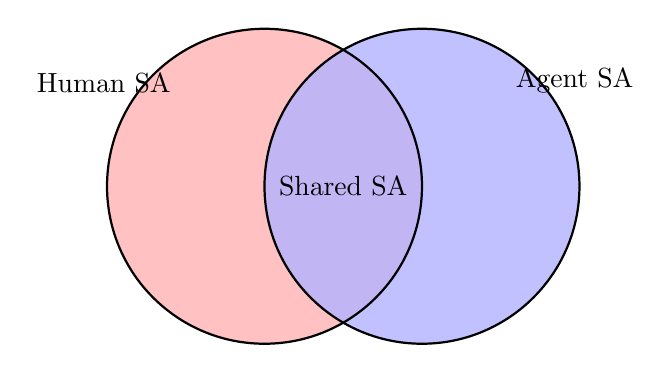
\begin{tikzpicture}
        % Left circle (Human SA)
        \fill[red!30, opacity=0.8] (-1,0) circle (2);
        % Right circle (Agent SA)
        \fill[blue!30, opacity=0.8] (1,0) circle (2);

        % Borders
        \draw[thick] (-1,0) circle (2) node[above left=1.5cm] {Human SA};
        \draw[thick] (1,0) circle (2) node[above right=1.5cm] {Agent SA};

        % Label overlap
        \node at (0,0) {Shared SA};
		\end{tikzpicture}
		\caption{Venn diagram illustrating Team Situation Awareness (Team SA) with the overlapping individual SA of the human pilot and the autonomous agent representing Shared SA.}
		\label{fig:team-sa-venn}
	\end{figure}

	\subsubsection{Interdependence Analysis}
	Interdependent Analysis is a work analysis method part of the coactive design process that helps improve collaboration between humans and machines by identifying key interdependence relationships that are essential for effective teamwork \parencite{johnson_coactive_2014}. It also defines requirements for tasks that involve interdependence, ensuring successful cooperation. This framework consists of three main parts: (1) joint activity modeling, (2) interdependence assessment, and (3) workflow analysis. These components help guide the design of systems for more effective teamwork, particularly in human-autonomy teams \parencite{johnson_understanding_2018} \textbf{to be moved in SotA}.
	To define human and autonomy role for our case study we have performed an Interdependence Analysis. This tool's most powerful feature is its ability to map different teaming options at the beginning of the design process, as opposed to a single function allocation solution. The output of an IA gives:
	\begin{itemize}
		\item a sequential hierarchical breakdown of tasks and capacities required to perform the scenario (section 1 of Table~\ref{table:IA})
		\item Different teaming alternatives, especially in our case the dyad human-agent with human as main performer of the activity and agent as supporter or conversely agent as the main performer and human as the supporter (section 2 of Table~\ref{table:IA}).
		\item A visualization of possible workflows for the team to carry-out the activity, depending on the team alternative, required, and opportunistic interdependence relationship (section 3 of Table~\ref{table:IA}).
		\item A list of \textbf{Observability, Predictability, and Directability} requirements to ensure proper collaboration for the human-autonomy team (Table~\ref{table:OPD}).
	\end{itemize}
	The output of the GDTA was used to facilitates the IA, the goal hierarchy served to create the Joint Activity Graph, which is a hierarchical task decomposition of the activity, and the information requirements also guided the fine-level task definition. (the full IA table is in Appendix~\ref{table:all-IA})
	
	\begin{table}[H]
		\centering
		\caption{Interdependence Analysis table excerpt, see Table~\ref{table:color-key} for color key details}
		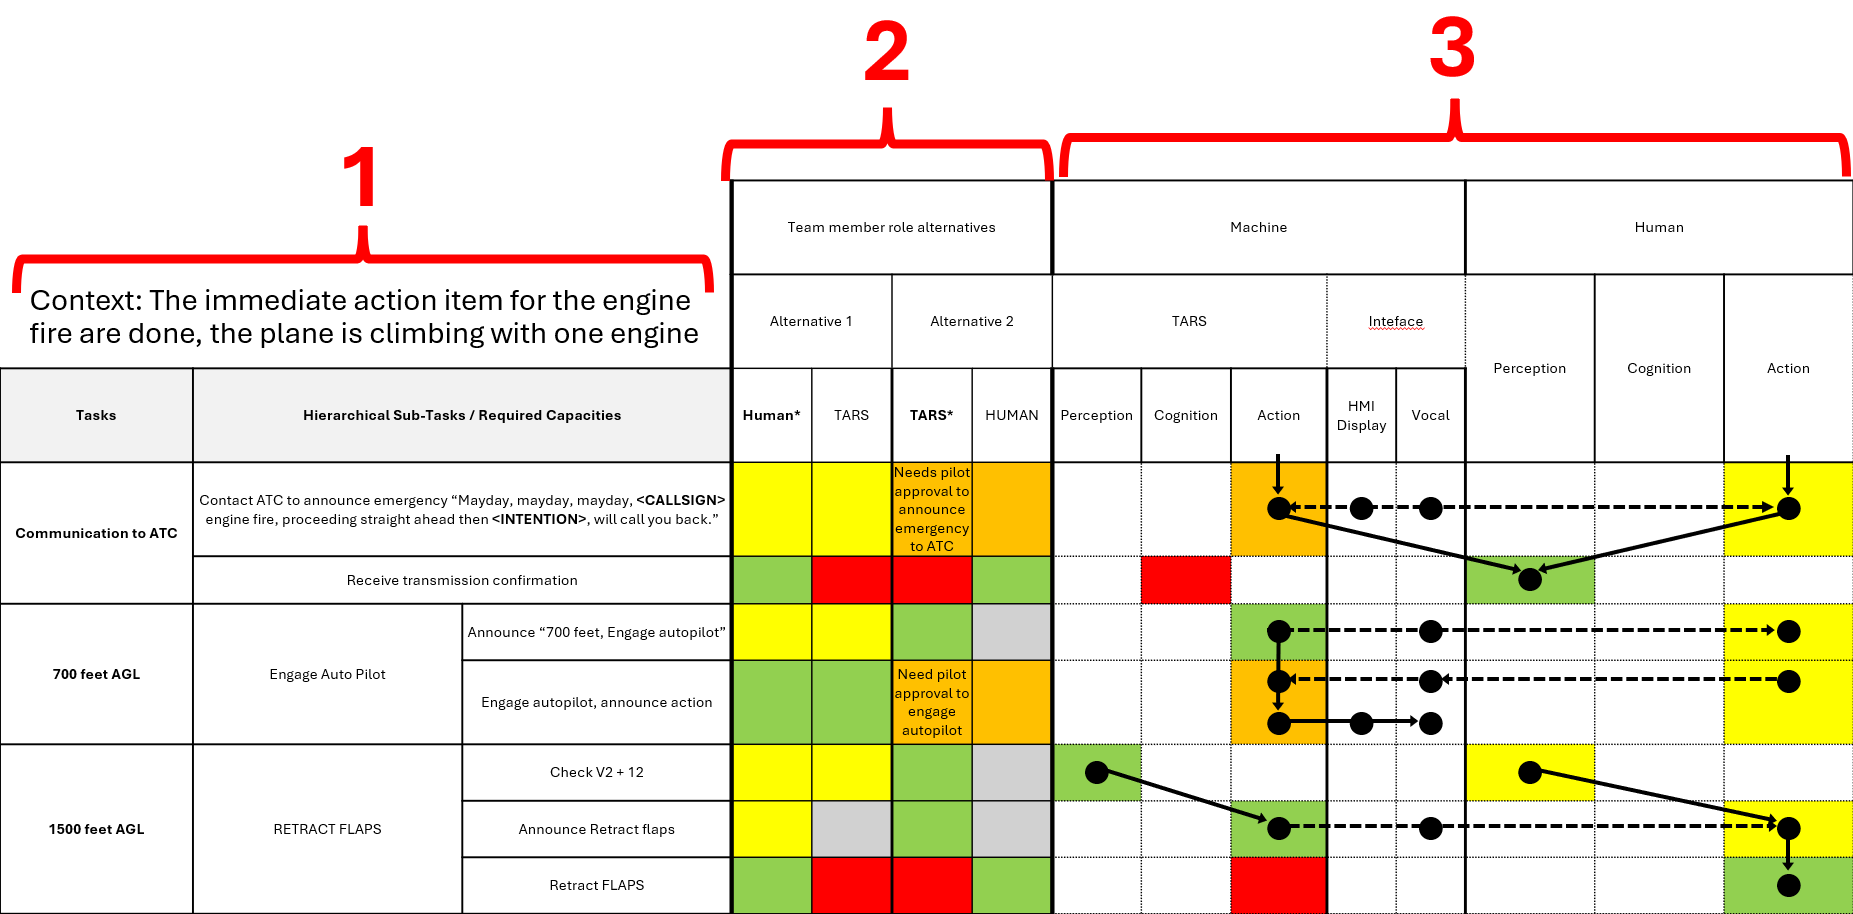
\includegraphics[width=1\textwidth]{images/IA-table.png}
		\label{table:IA}
	\end{table}

	\begin{table}[H]
		\centering
		\caption{Observability, Predictability, Directability requirements excerpt}
		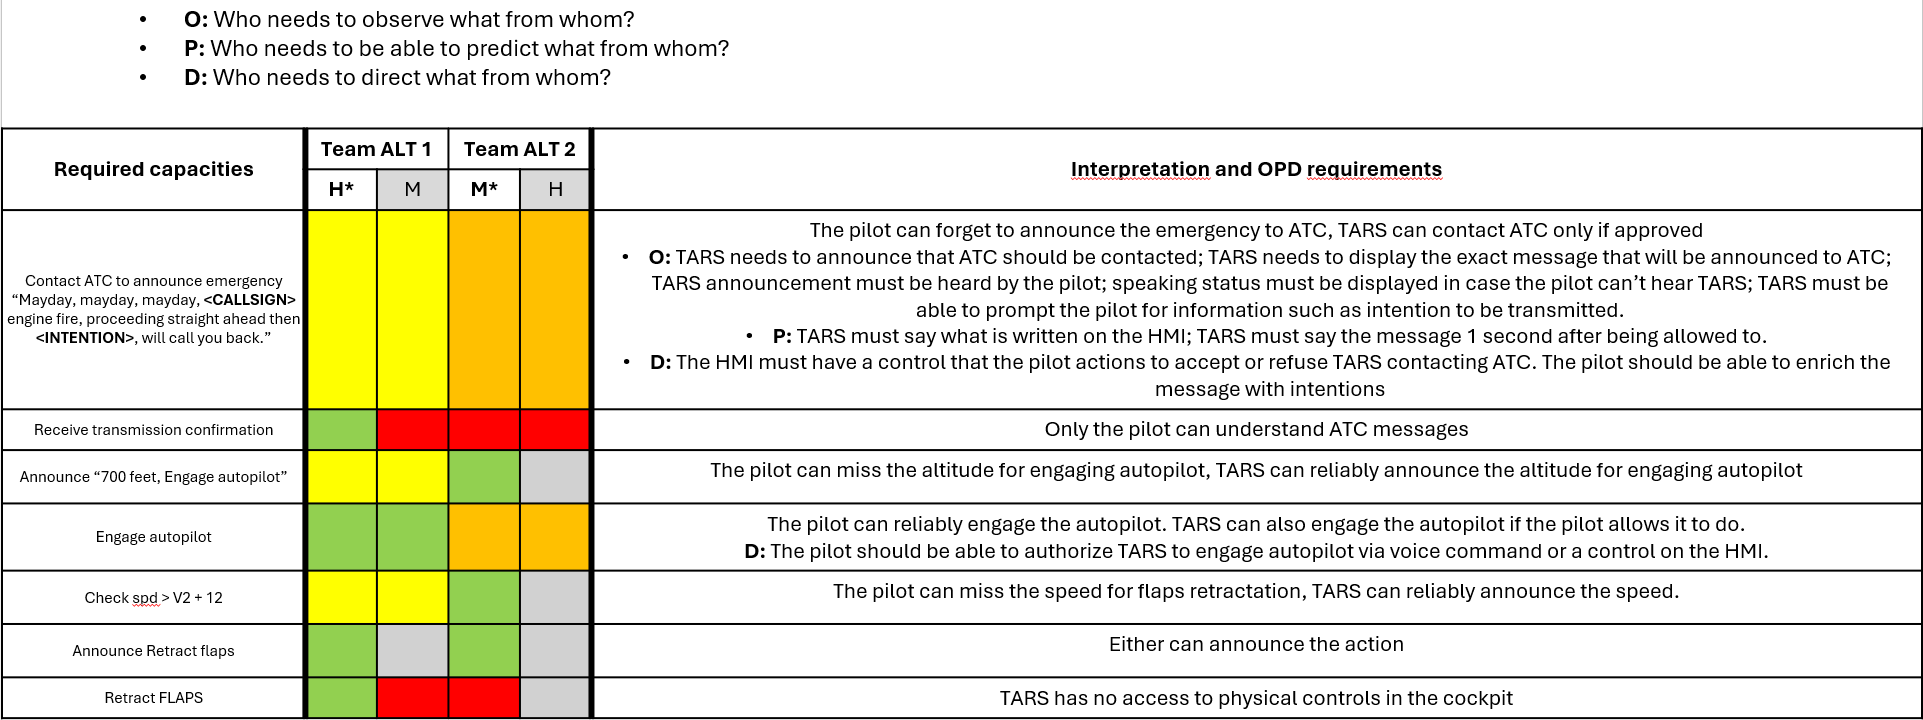
\includegraphics[width=1\textwidth]{images/OPD_table.png}
		\label{table:OPD}
	\end{table}

	The phase 1 and objectives~\ref{obj:1a} and~\ref{obj:1b} have been completed. A chapter titled \textit{"All hands on deck: Case study for Human-Autonomy Teaming (HAT) for Future Commercial Aviation Concepts of Operations"} in the \textit{Handbook of Socio-Technical Systems -- A Human Systems Integration Approach} has been submitted detailing the use-case scenario and methodological approach, it is currently being reviewed.

	\subsection{Phase 2: Cognitive modeling and agent development}

	\begin{figure}[H]
		\centering
		% First logo
		\begin{minipage}[b]{0.3\textwidth}
			\centering
			\raisebox{2mm}{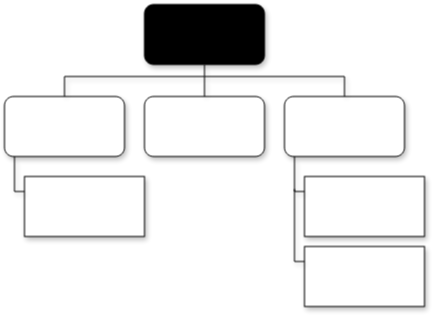
\includegraphics[width=0.9\textwidth]{images/hierarchy_diagram.png}}
		\end{minipage}
		% Second logo
		\begin{minipage}[b]{0.3\textwidth}
			\centering
			
\includegraphics[width=0.6\textwidth]{images/workflow_icon.png}
		\end{minipage}
		% Third logo
		\begin{minipage}[b]{0.3\textwidth}
			\centering
			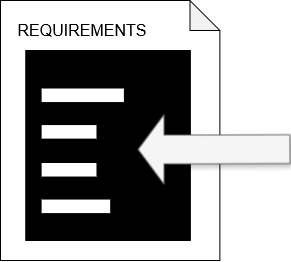
\includegraphics[width=0.8\textwidth]{images/requirements.png}
		\end{minipage}
		\caption{Output of phase 1 - goal hierarchy, task workflow, information \& OPD requirements.}
		\label{fig:logos}
	\end{figure}

	The phase 1 allowed us to delineate the design domain and list detailed information as well as teaming requirements that will be useful for the modelling and agent design phase, especially:

	\begin{itemize}
		\item The goal hierarchy will be used for the task structure of the cognitive model and the agent, each goal from the GDTA will be implemented in the cognitive model using the goal module of the ACT-R architecture, responsible for holding the current goal or focus of attention of the model. Likewise, agent-side, the goal hierarchy will be represented as a structure containing states and transitions akin to a Finite State Machine (FSM)
		\item Workflows from the IA will be used as an input to a module responsible for the task allocation between the model and the agent, for each workflow, this "dispatcher" module will effectively activate or inhibit actions for the model and agent.
		\item Information requirements will be used to program that both the model and agent attend to the relevant elements of the environment for the task at hand. It will also be used for SA assessment, as the cognitive model can be asked to answer questions regarding the value/status of relevant information for the task, and information representation of the agent can be inspected at any time, thus the alignment in SA can be approximated by the difference in situation representation for both teammates. OPD requirements will be individually assessed during simulation by observing team behavior.
	\end{itemize}

	\subsubsection{QN-ACTR and SEEV}
	\label{qn-actr-seev}
	The cognitive model of the single pilot will be implemented using the QN-ACTR architecture, integrating a simplified SEEV model to capture attention allocation dynamics and level 1 situation awareness (SA). Based on the output from Phase 1, operational documentation, and available training materials, an initial model of an expert pilot operating a Cessna Citation Mustang will be developed. The model will simulate routine procedural execution, following Standard Operating Procedures (SOPs) and checklists for the takeoff phase, \textbf{without any assistance from an autonomous agent} (baseline model).

	The model will be connected to X-Plane 11 in a closed-loop simulation, receiving real-time aircraft and environment data and issuing control inputs directly to the simulator via UDP. Once the baseline model can effectively navigate the scenario, it will be extended to collaborate with the autonomous agent, enabling it to observe and direct the agent's actions.
	
	The model will be implemented in Lisp and integrated into the QN-ACTR platform, with necessary adjustments to the platform to ensure appropriate input/output handling with X-Plane 11. Development will build upon the QN-ACTR takeoff model by Xu and colleagues \parencite{xu_modeling_2021}, which currently models a single-pilot normal takeoff procedure in a Cessna 172 aircraft.
	
	The SEEV model will be applied to determine the probability of the pilot allocating attention to relevant Areas of Interest (AOIs) in the cockpit and external environment. The SEEV parameters—Salience, Effort, Expectancy, and Value—will initially adopt the coefficient weights proposed by Wang et al. \parencite{wang_real-time_2024}, whose model was tuned for a similar scenario (engine failure at takeoff in Single Pilot Operations). Their configuration defines seven AOIs: (1) Primary Flight Display (PFD), (2) Navigation Display (ND), (3) Engine/Warning Display (E/WD), (4) System Display (SD), (5) Central Console, (6) Flight Manual, and (7) Outside Window.
	
	The attention probability ($P(AOI)$) towards each AOI will be computed using a simplified version of SEEV, where Effort and Salience parameters are discounted, following common practices in driving and aviation simulator studies \parencite{rehman_phd_thesis}. This is justified by the reduced visual angles and minimal scanning effort required in such setups. The attention allocation formula is defined in Equation~\ref{eq:VA_AOI}: %check this ref, not only cite Rehman's thesis.
	
	\begin{equation}
		VA_{AOI} = \sum_{t=1}^{n} (Ex_t) (R_t) (P_t)
		\label{eq:VA_AOI}
	\end{equation}
	Here, $VA_{AOI}$ is the raw attention value for an AOI, $t$ indexes across $n$ tasks, $Ex_t$ is the Expectancy of the AOI for task $t$, $R_t$ is its Relevance, and $P_t$ is the Priority of task $t$. The combined effect of $R_t$ and $P_t$ represents the "Value" factor in the SEEV model.
	
	The resulting $VA_{AOI}$ values are normalized to generate probabilistic attention weights across all AOIs. Monte Carlo simulations will be used to stochastically determine gaze allocation over time.
	
	The model accounts for both attentional and memory constraints: attention allocation drives what information enters the cognitive system, while ACT-R's declarative memory mechanisms (e.g., memory decay and activation thresholds) govern subsequent retention and retrieval. In QN-ACTR, activation levels of chunks representing critical elements must exceed a threshold to contribute to Level 1 SA (perception-based SA). Consequently, Level 1 SA in this model emerges from the interaction between visual attention (SEEV) and cognitive memory dynamics (ACT-R). The framework is presented in Figure~\ref{fig:qn-actr-seev}

	\begin{figure}[H]
    \centering
    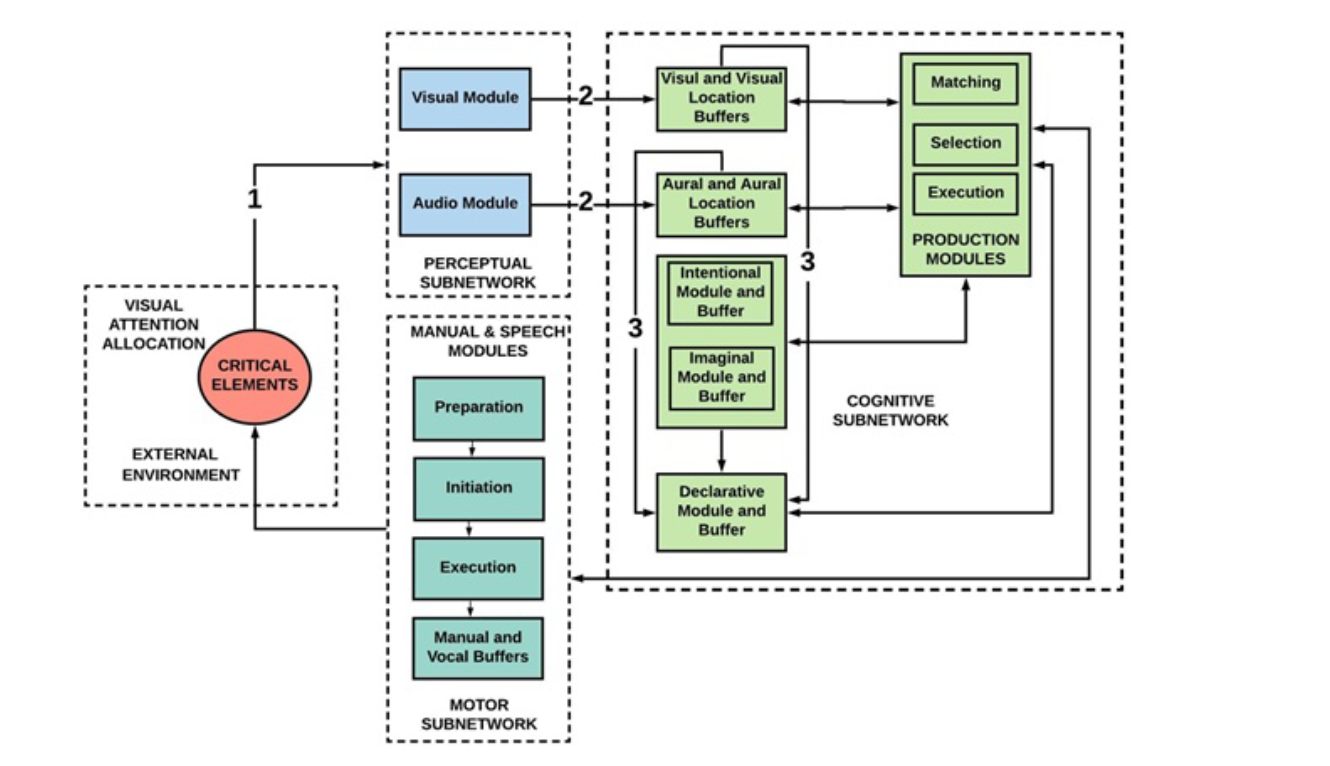
\includegraphics[width=0.9\textwidth]{./images/qn-actr-sa-synoptic.png}
    \caption{Overview of the QN-ACTR-SEEV framework. Stages 1-3 (marked on the lines in the figure) signify the different cognitive processes necessary in the acquisition and maintenance of Level 1 SA. Adapted from Rehman (2020) \parencite{rehman_phd_thesis}.}
    \label{fig:qn-actr-seev}
	\end{figure}


	
	\subsubsection{Agent design}
	A functional prototype of the Autonomous Agent (AA) system will be developed in parallel with the cognitive model to meet the previously defined requirements. The prototype will be deployed as a tablet application interfacing with the flight simulator and positioned within the cockpit environment.

	The AA is implemented as a modular and reactive software component designed to assist the pilot in managing the flight scenario. The agent adopts a nested Finite State Machine (FSM) architecture, employing the state pattern, to organize its behavior into a structured hierarchy of states and substates. Each state encapsulates a specific procedural phase of the scenario, with transitions triggered by defined environmental conditions.
	
	This design was selected to reflect the deterministic and highly procedural characteristics of the flight scenario. The agent does not incorporate deliberative planning or uncertainty handling; rather, it functions as a partial Wizard of Oz system. Its purpose is to emulate the expert-like behavior of an AI system that executes preprogrammed actions in response to situational cues.
	
	The AA system is composed of the following modules: 
	\begin{itemize} 
		\item \textbf{State Hierarchy:} A layered structure of states and nested substates representing sequential and conditional phases of the flight (e.g., "Takeoff Roll" $\rightarrow$ "Engine-Out Emergency Procedure" $\rightarrow$ "Communicate with ATC").
		\item \textbf{State Manager:} A supervisory module responsible for managing transitions between states based on predefined transition rules.
		\item \textbf{Action Layer:} A set of atomic actions (e.g., "Verify engine instruments", "Declare emergency to ATC") executed when specific states or substates become active.
		\item \textbf{Status Monitoring:} A continuous input channel from the flight simulator (X-Plane 11) used to assess scenario conditions and update the agent's internal state. 
	\end{itemize}
	
	The nested FSM structure provides a modular and scalable framework, ensuring ease of maintenance and facilitating the alignment between the agent's reactive behavior and the cognitive model's procedural logic.

	\begin{figure}[H]
		\centering
		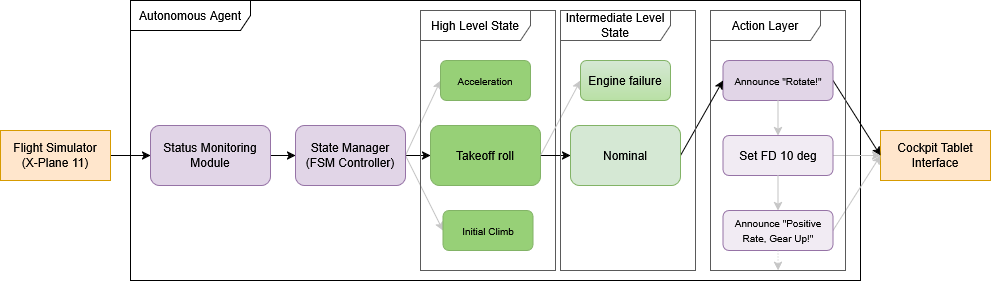
\includegraphics[width=1.0\textwidth]{./images/AA_synoptic.png}
		\caption{AA Synoptic diagram}
		\label{fig:aa_synoptic}
	\end{figure}
	
	\subsubsection{System architecture}
	The whole system architecture consists of three principal components: the Cognitive Model (QN-ACTR + SEEV), the AA, and the Task Dispatcher. These components operate within the same local network.

	\begin{itemize} 
		\item \textbf{Task Dispatcher:} A central module responsible for allocating tasks between the cognitive model (representing the human pilot) and the AA (the virtual copilot). The dispatcher can be thought of representing the Human-Autonomy pre-flight briefing. It activates or inhibit tasks for each member of the team, ensuring overall coherence between entities for effective collaboration to achieve the shared set of goals. It also automates simulation batches.
		\item \textbf{Cognitive Model:} The QN-ACTR+SEEV model simulates the pilot's cognitive processes, including level 1 situation awareness, memory dynamics, and attention allocation. It is capable of both executing tasks directly and interacting with the AA.
		\item \textbf{Autonomous Agent (AA):} As outlined earlier, this agent handles delegated tasks from the dispatcher and takes direct action in the simulation environment to assist the pilot.
	\end{itemize}

	The system leverages the \textbf{Ingescape ecosystem} to connect distributed modules seamlessly:
	\begin{itemize}
		\item \textbf{Black-box agents:} Each software module (dispatcher, cognitive model, AA agent) is implemented as an independent black box with defined input/output ports.
		\item \textbf{ZeroMQ-based messaging:} Ingescape abstracts communication, enabling asynchronous and decoupled messaging between components.
		\item \textbf{Simulation Interface:} Both the AA agent and the cognitive model exchange real-time data with X-Plane 11 and between themselves, ensuring they operate with a synchronized and shared representation of the environment orchestrated by the ingescape platform.
	\end{itemize}

	This architecture enables flexible experimentation, including various teaming strategies (e.g., autonomous agent as backup or co-pilot), and modular upgrades to individual system components, see Figure~\ref{fig:ingescape_platform}.

	\begin{figure}[H] 
		\centering
		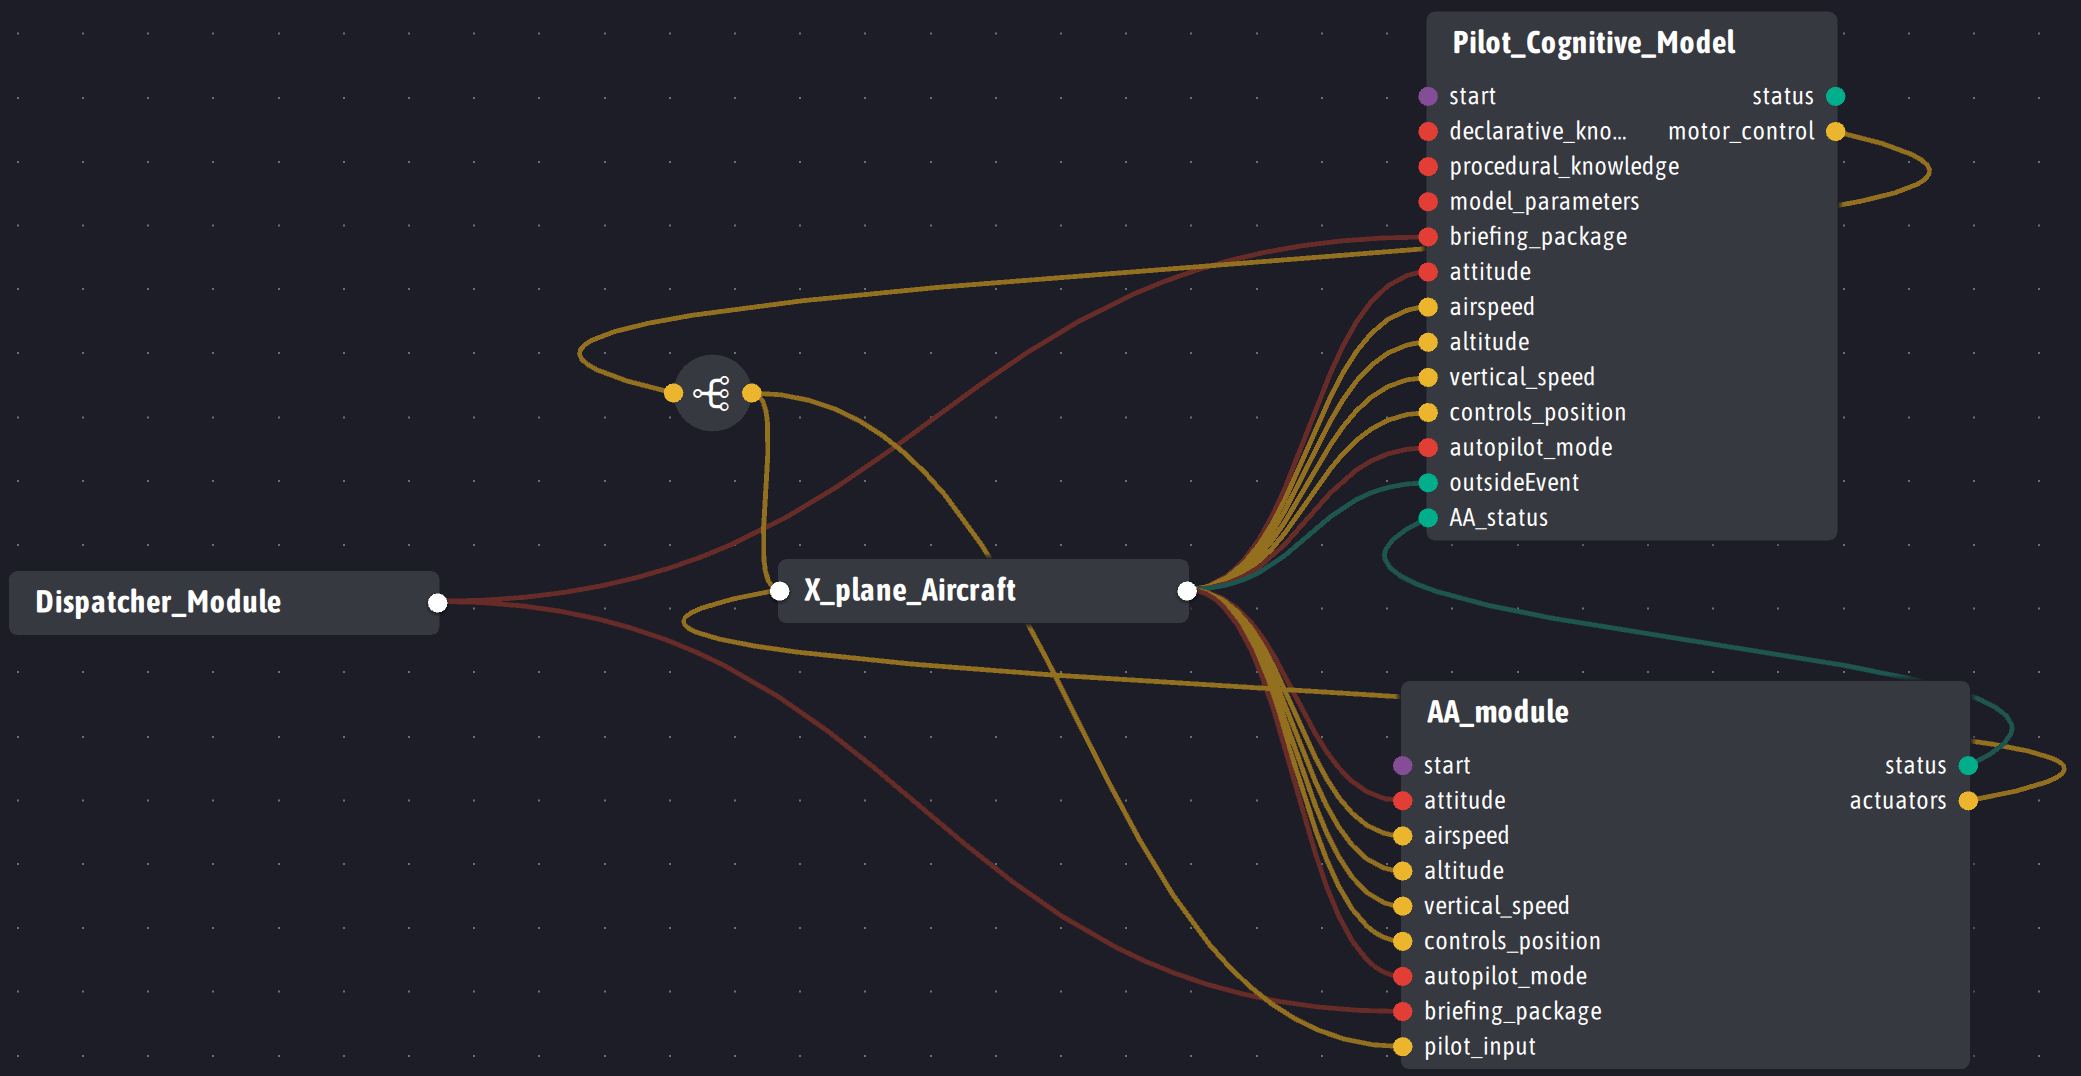
\includegraphics[width=1.0\textwidth]{./images/ingescape_platform.png}
		\caption{system architecture overview from the ingescape platform}
		\label{fig:ingescape_platform}
	\end{figure}

	\subsubsection{Scenario \& Simulation}
	We constructed the scenario based on checklists, standard operating procedures (SOPs), training material, and feedback from subject matter experts of the Cessna Citation Mustang. This aircraft is single-pilot certified, meaning that the required procedures are currently performed by either a single pilot or a two-pilot crew. This aspect eased the construction of the cognitive model, because a baseline single-pilot operation (SPO) already exists, eliminating the need to invent new procedures. We ensured that our scenario remains as close to operational reality as possible, it is depicted in~\ref{fig:scenario_detailed}.

	\begin{figure}[H]
		\centering
		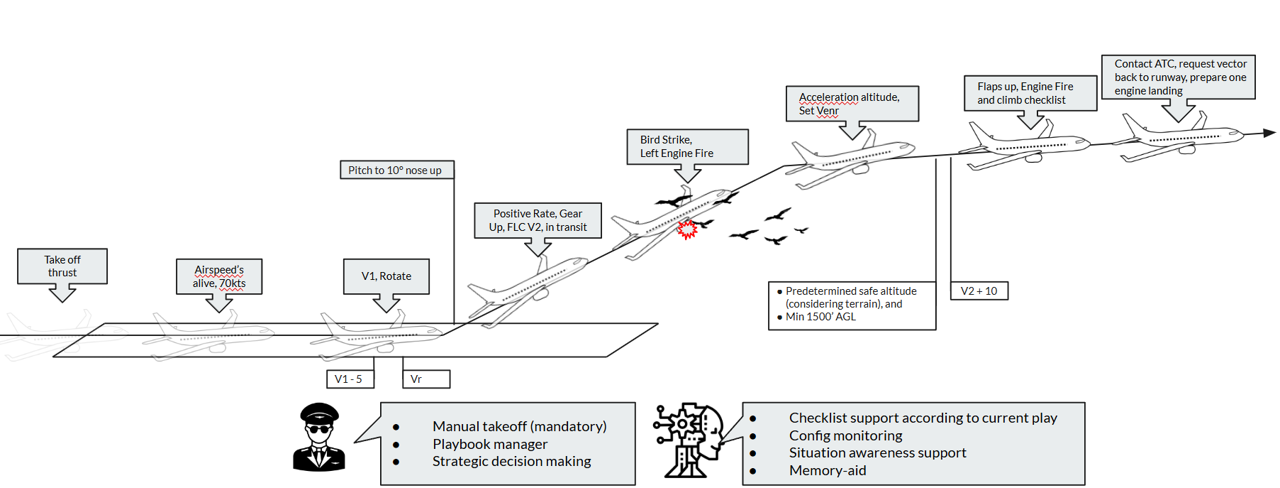
\includegraphics[width=1.0\textwidth]{./images/scenario_detailed.png}
		\caption{Takeoff scenario detailed}
		\label{fig:scenario_detailed}
	\end{figure}

	Upon completing the development of both the cognitive model and the autonomous agent, we will enter the simulation phase to gather data. The experiment will involve two independent variables, each designed to examine different aspects of human-autonomy teaming in aviation represented by 5 different dependent variables, all synthesized in Table~\ref{tab:variables}.
	
	\textbf{Independent Variables}
	\begin{itemize}
	\item \textbf{IV1 : Teaming Configuration}:
	\begin{itemize}
	\item \textbf{Baseline condition}: Cognitive model alone in SPO
	\item \textbf{Low teaming}: Using only the required teaming interdependence ()
	\item \textbf{High teaming}: Using every required and opportunistic teaming interdependence
	\end{itemize}
	\item \textbf{IV2 : Scenario Variations}:
	\begin{itemize}
	\item \textbf{Nominal Condition}: No bird strike
	\item \textbf{Non-Nominal Conditions}:
	\begin{itemize}
	\item Bird strike and engine failure before V1 (Rejected Takeoff scenario)
	\item Bird strike and engine failure after V1 (Engine failure in flight scenario)
	\end{itemize}
	\end{itemize}
	\end{itemize}
	
	\textbf{Dependent Variables}
	\begin{itemize}
	\item \textbf{DV1 : Situation Awareness (SA)}:
	\begin{itemize}
	\item Assessed through the SAGAT (Situation Awareness Global Assessment Technique) methodology at various points in the scenario.
	SAGAT questions are derived from the GDTA (Goal-Directed Task Analysis) information requirements and will be probed to the cognitive model by pausing the simulation at predefined moments.
	\item The autonomous agent's current situation representation will be retrieved simultaneously by inspecting relevant flight parameters values as defined by the information requirements.
	\end{itemize}
	\item \textbf{DV2 : Workload}:
	\begin{itemize}
	\item Estimated workload levels are automatically output by QN-ACTR. The architecture considers ACT-R modules and buffers as servers and uses "Expected Utilization as a workload index to capture the impact of time stress. Expected Utilization is defined as the ratio of the server processing time required by task demands to the total available task time" \parencite{cao_modelling_2015}.
	\begin{equation}
		Expected\ Utilization = \frac{Time_{required}}{Time_{total}} 
	\end{equation}
	Workload is assumed to have a linear relationship with the overall expected utilisation (OEU) averaged from all servers that have non-zero service time
	\end{itemize}
	\item \textbf{DV3 : Performance Metrics}:
	\begin{itemize}
	\item Time to return to a nominal flight condition following the bird strike:
	\begin{itemize}
	\item Rejected takeoff: Reaction time to initiate the rejected takeoff action.
	\item Engine failure after takeoff: Time to execute the emergency procedures and checklist.
	\end{itemize}
	\end{itemize}
	\item \textbf{DV4 : Attention Allocation and Gaze Behavior}:
	\begin{itemize}
	\item The cognitive model's gaze patterns and attention allocation toward Areas of Interest (AoIs) will be analyzed, including fixation count and total gaze time per AoI.
	\end{itemize}
	\item \textbf{DV5 : Teaming Effectiveness Evaluation}:
	\begin{itemize}
	\item Systematic validation of teaming requirements (except Predictability which would require modelling of anticipation --- SA level 3 --- which is outside of the scope of this thesis):
	\begin{itemize}
	\item \textbf{Observability}: The agent's actions and state must be observable to the human pilot.
	\item \textbf{Directability}: The human pilot must be able to direct the agent effectively.
	\end{itemize}
	\end{itemize}
	\end{itemize}
	
	\textbf{Simulation Repetitions and Statistical Analysis}
	Given the stochastic nature of the cognitive model's attention allocation module (based on the SEEV model), each condition will be the same number of times than participants recruited for HITLS.

	\textbf{Hypotheses :}
	\begin{enumerate}[label=\textbf{H\arabic* :}]
	\label{hypotheses}
	\item \textbf{Workload predicted level}: No teaming $>$ Low teaming $>$ High teaming
	\item \textbf{Situation Awareness level}: No teaming $<$ Low teaming $\approx$ High teaming (no significant differences between teaming configurations)
	\item \textbf{Team SA alignment}: Low teaming $<$ High teaming. Which means that in high teaming condition, the cognitive model's critical information representation's value should closely match the autonomous agent's
	\item \textbf{Performance level}: No teaming $<$ Low teaming $<$ High teaming
	\item \textbf{Fixation count and gaze time on the autonomy's HMI}: Low teaming $<$ High teaming
	\end{enumerate}
	Additionally, we anticipate being able to systematically validate the \textbf{Observability} and \textbf{Directability} requirements during the simulation phase.
	
	\begin{table}[h]
		\centering
		\caption{Independent and Dependent Variables Overview}
		\renewcommand{\arraystretch}{1.3}
		\resizebox{\textwidth}{!}{ % This scales the table to fit within text width
		\begin{tabular}{|l|l|}
			\hline
			\textbf{Independent Variables} & \textbf{Levels} \\
			\hline
			\textbf{Teaming Configuration} & \begin{tabular}[c]{@{}l@{}}Baseline: Cognitive model alone in SPO \\ Low: Only required teaming interdependence \\ High: Required + opportunistic interdependence\end{tabular} \\
			\hline
			\textbf{Scenario Variations} & \begin{tabular}[c]{@{}l@{}}Nominal: No bird strike \\ Non-Nominal: \\ - Bird strike + engine failure before V1 (Rejected Takeoff) \\ - Bird strike + engine failure after V1 (Engine failure after takeoff)\end{tabular} \\
			\hline
			\textbf{Dependent Variables} & \textbf{Measurement Approach} \\
			\hline
			\textbf{Situation Awareness (SA)} & \begin{tabular}[c]{@{}l@{}}SAGAT score \\ Agent's situation representation captured simultaneously\end{tabular} \\
			\hline
			\textbf{Cognitive Model Workload} & \begin{tabular}[c]{@{}l@{}}Output from QN-ACTR Expected Utilization\end{tabular} \\
			\hline
			\textbf{Performance Metrics} & \begin{tabular}[c]{@{}l@{}}(Rejected takeoff): Reaction time to initiate procedure \\ (Engine failure after takeoff): Time for completing emergency procedures\end{tabular} \\
			\hline
			\textbf{Attention Allocation and Gaze Behavior} & \begin{tabular}[c]{@{}l@{}} Fixation count and gaze time on Autonomous agent's HMI\end{tabular} \\
			\hline
			\textbf{Teaming Effectiveness Evaluation} & \begin{tabular}[c]{@{}l@{}}Validation of teaming requirements: \\ - Observability: Agent's actions must be observable \\ - Directability: Pilot must be able to direct the agent\end{tabular} \\
			\hline
		\end{tabular}
		}
		\label{tab:variables}
	\end{table}

	The phase 2 will complete objectives~\ref{obj:2a}, \ref{obj:2b}, \ref{obj:2c} and \ref{obj:2d}. We expect to publish a journal article detailing the coupling of a situation awareness cognitive model and an autonomous agent in a closed-loop simulation study, as well as simulation results and how they can be used to iterate the design of the agent and HMI. According to our research, this is a novel contribution, our goal is to publish in a Human-Computer interaction / human factors research journal, preferably an issue on Human Performance Modelling / cognitive modelling.

	\subsection{Phase 3: Human-In-The-loop simulation studies}

	\subsubsection{Scenario}
	The scenario for the Human-in-the-Loop Simulation (HITLS) study is identical to the one executed by the cognitive model. It involves the same aircraft type, cockpit layout, SOPs, route, weather conditions, and emergency procedures to ensure consistency and comparability between computer simulation and human experiments.

	\subsubsection{Equipment}
	The study will be conducted in the full-flight simulator at Polytechnique Figure~\ref{fig:simu_cockpit}A, which represents the cockpit layout of a Beechcraft Baron G58 equipped with Garmin G1000 avionics. This setup is highly similar to the Cessna Citation Mustang's cockpit Figure~\ref{fig:simu_cockpit}B, ensuring minimal differences in interface and procedural interactions. A camera-based eye tracker (spec ??) will be integrated into the simulator to capture gaze behavior, with defined Areas of Interest (AoIs) matching those in the cognitive model's SEEV module (\ref{qn-actr-seev}).

	\begin{figure}[H]
		\centering
		% First logo
		\begin{minipage}[b]{0.50\textwidth} % Adjusted width
			\centering
			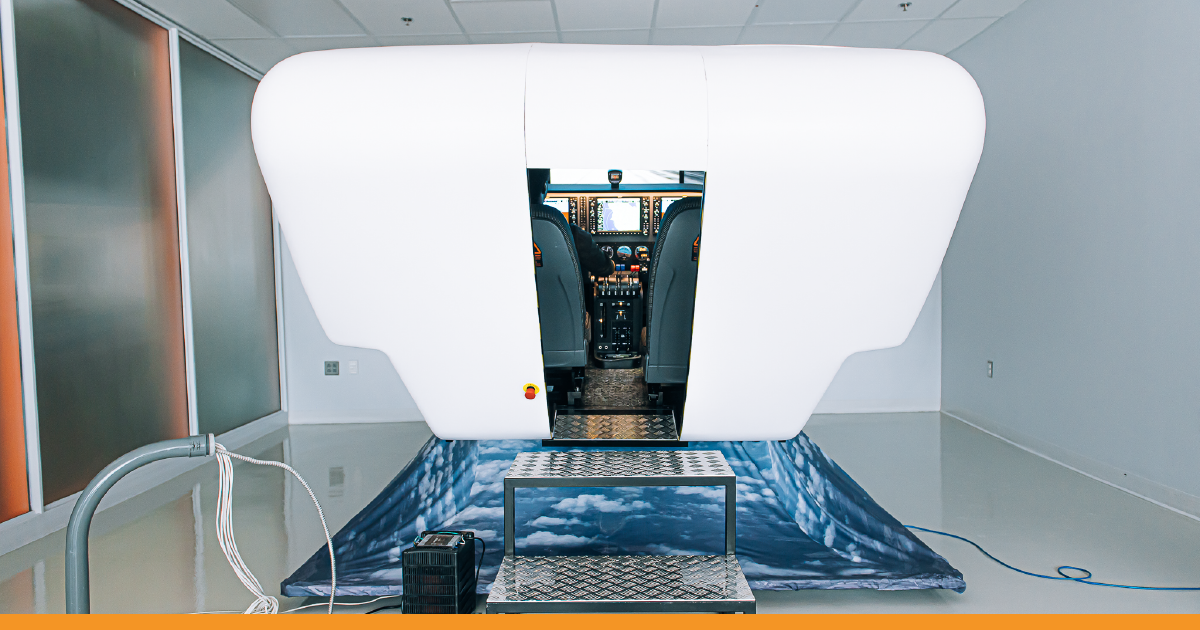
\includegraphics[width=\textwidth]{images/poly_simu.png}
		\end{minipage}
		\hfill % Adds space between the two figures
		% Second logo
		\begin{minipage}[b]{0.45\textwidth} % Adjusted width
			\centering
			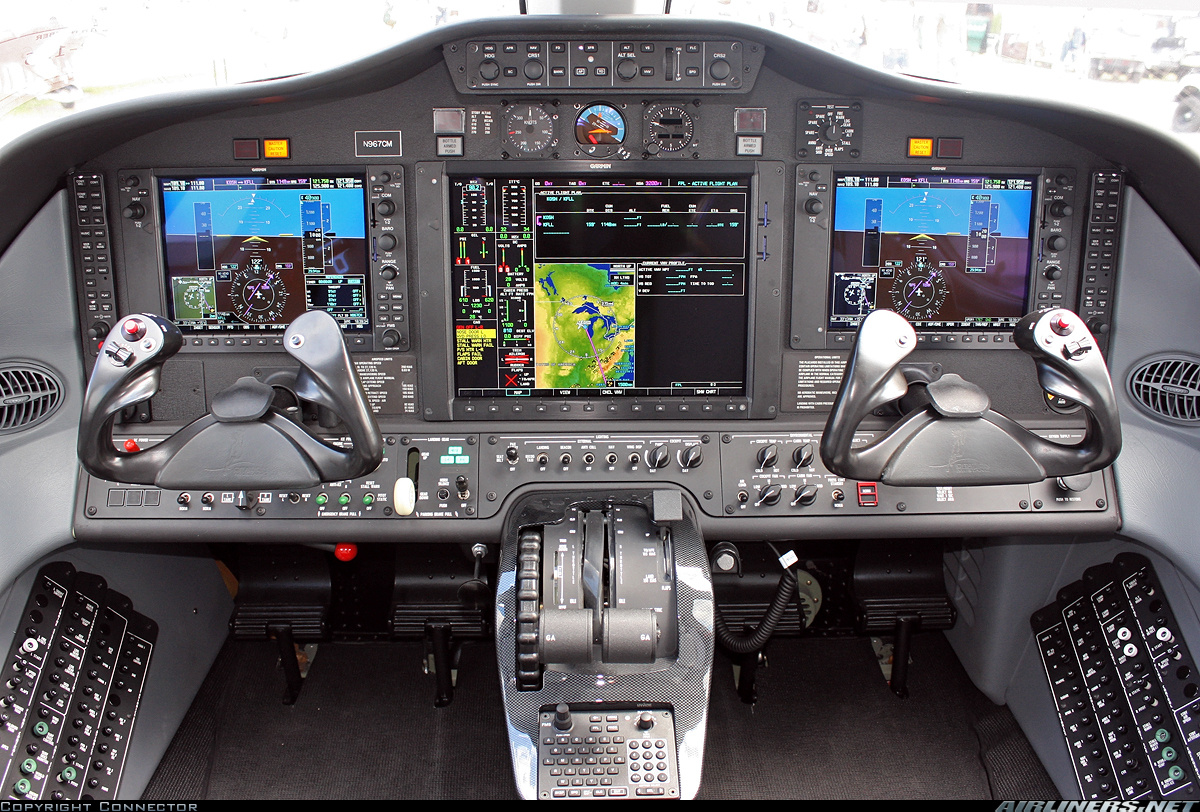
\includegraphics[width=\textwidth]{images/mustang_cockpit.jpg}
		\end{minipage}
		\caption{A: Polytechnique's simulator and B: Cessna Citation Mustang cockpit.}
		\label{fig:simu_cockpit}
	\end{figure}
	

	\subsubsection{Participants}
	We will recruit at least 15 pilots holding a Commercial Pilot License (CPL) with prior experience in multi-crew operations. This ensures that participants are familiar with the teamwork dynamics necessary for human-autonomy teaming studies.

	\subsubsection{Protocol}
	Each pilot will undergo a formal pre-flight briefing phase before each scenario. The briefing will adhere to aviation standards, covering:
	\begin{itemize}
		\item Route and weather conditions
		\item Departure and emergency procedures
		\item Communication and automation plans
		\item Human-AI crew roles
		\item Aircraft performance 
	\end{itemize}
	This briefing phase is crucial, as identified in the GDTA and pilot interviews, participants emphasized that "\textit{The Plan}" established during briefing dictates the crew's actions and cooperation throughout the flight. Pilots only deviate from \textit{The Plan} in unexpected situations, and a bird strike and engine failure at takeoff is considered during the briefing, reinforcing the need for a structured pre-flight preparation.

	Participants will first complete a familiarization scenario to reduce training bias. This phase introduces them to Polytechnique's simulator and the autonomous agent's interface. During the scenario, the simulator will be paused at predefined moments to administer SAGAT probes assessing the pilot's situation awareness. Pilot's gaze behavior will be continuously recorded.
	Given that Predictability is the only OPD requirement not covered by the cognitive model, special SAGAT probes will be asked to verify if pilots can anticipate the behaviour of the autonomous agent, thus validating this final set of requirements.
	After each scenario, pilots will complete:

	\begin{itemize}
		\item NASA-TLX: A standardized workload assessment questionnaire.
		\item SUS (System Usability Scale): Evaluating the usability of the human-agent interface. 
	\end{itemize}

	After every scenarios, pilots will engage in a semi-structured debriefing interview discussing:

	\begin{itemize}
		\item Trust in the autonomous agent,
		\item HMI design,
		\item Future human-autonomous agent crew roles,
		\item And any qualitative feedback,
	\end{itemize} 

	\subsubsection{Model validation and results}
	The HITLS serves two primary objectives. First, validating the model \ref{obj:3a}, by comparing simulated results with human empirical data, especially:
	\begin{enumerate}
		\item Simulated vs. empirical SAGAT scores.
		\item Simulated workload vs. NASA-TLX scores.
		\item Fixation count and fixation per AoI for both the cognitive model and human pilots.
		\item Compare simulated vs. empirical time to resolve emergencies in non-nominal scenarios. 
	\end{enumerate}
	Thus, we apply the same hypotheses than during computer simulation (\ref{hypotheses}) 
	More precisely, the model's goodness-of-fit will be assessed using Mean Absolute Percentage Error (MAPE), Root Mean Square Error (RMSE) and Coefficient of determination (R-squared).

	\begin{equation}
		RMSE = \sqrt{\frac{\sum_{i=1}^{n} \left(X_{human,i}-X_{model,i}\right)^2}{n} } 
	\end{equation}

	\begin{equation}
		MAPE = \frac{100}{n} \sum_{i=1}^{n} \left\lvert \frac{X_{human,i} - X_{model,i}}{X_{human,i}} \right\rvert 
	\end{equation}

	\begin{equation}
		R^2 = 1 - \frac{\sum_{i=1}^{n} (X_{human,i} - X_{model,i})^2}{\sum_{i=1}^{n} (X_{human,i} - \bar{X}_{human})^2}
	\end{equation}

	The second objective is to investigate non-modelable human factors \ref{obj:3b}, specifically predictability of autonomous agents's behaviour, trust, and usability aspects. We will also gather qualitative feedback on autonomous agent and HMI design and subjective responses regarding future human-autonomy crew roles.
	
	\section{Originality and Impact} % Section for originality and impact
	This project provides an advanced methodology for integrating collaborative autonomous systems into the cockpit, improving the safety and efficiency of Single Pilot Operations.
	
	\section{Risks assessment and mitigation}
	My risks
	
	\section{Resource management}
	My resources
	
	\section{Timeline}
	My timeline.

	\appendix
	\section{Goal-Directed Task Analysis}
	\label{appendix:GDTA}
	\subsection{Top-Level Goal hierarchy}

	\begin{figure}[H]
		\centering
		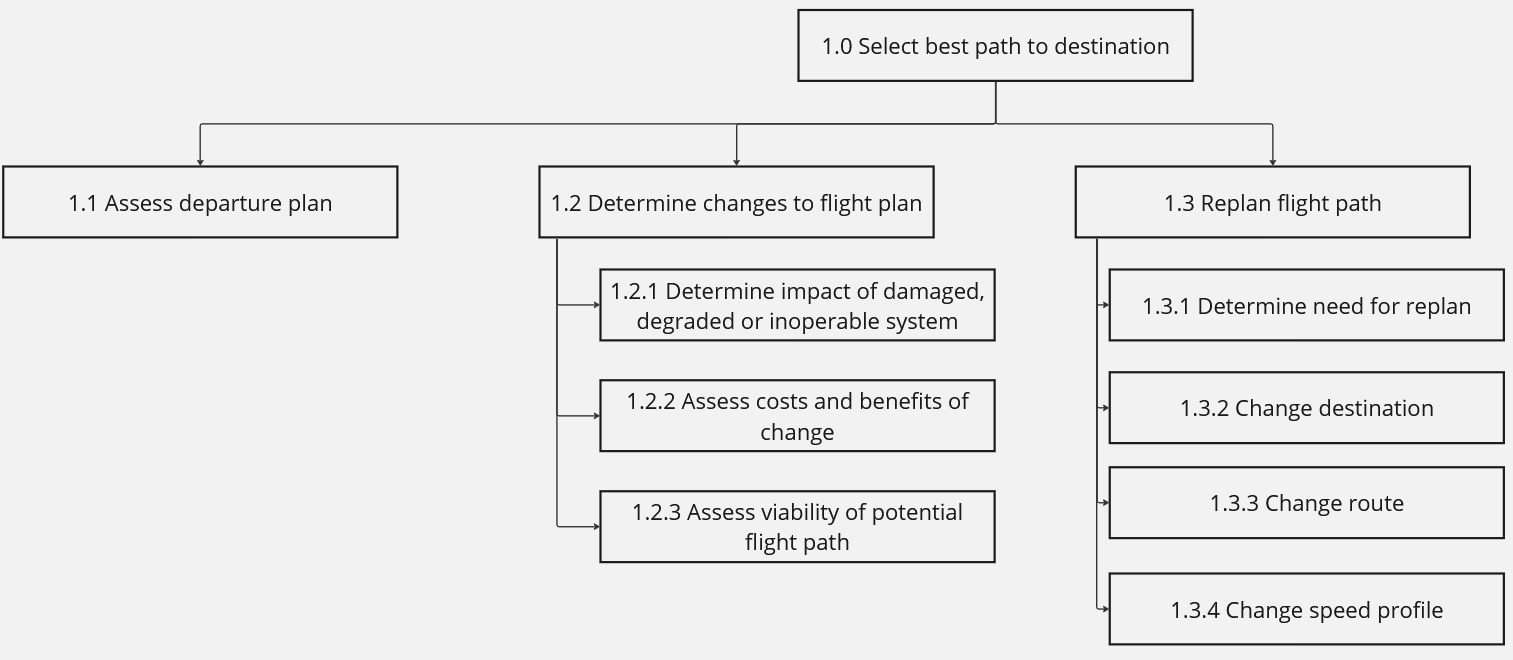
\includegraphics[width=1.0\textwidth]{./images/GDTA/top-goal-1.jpg}
		\label{gdta:top-1}
	\end{figure}

	\begin{figure}[H]
		\centering
		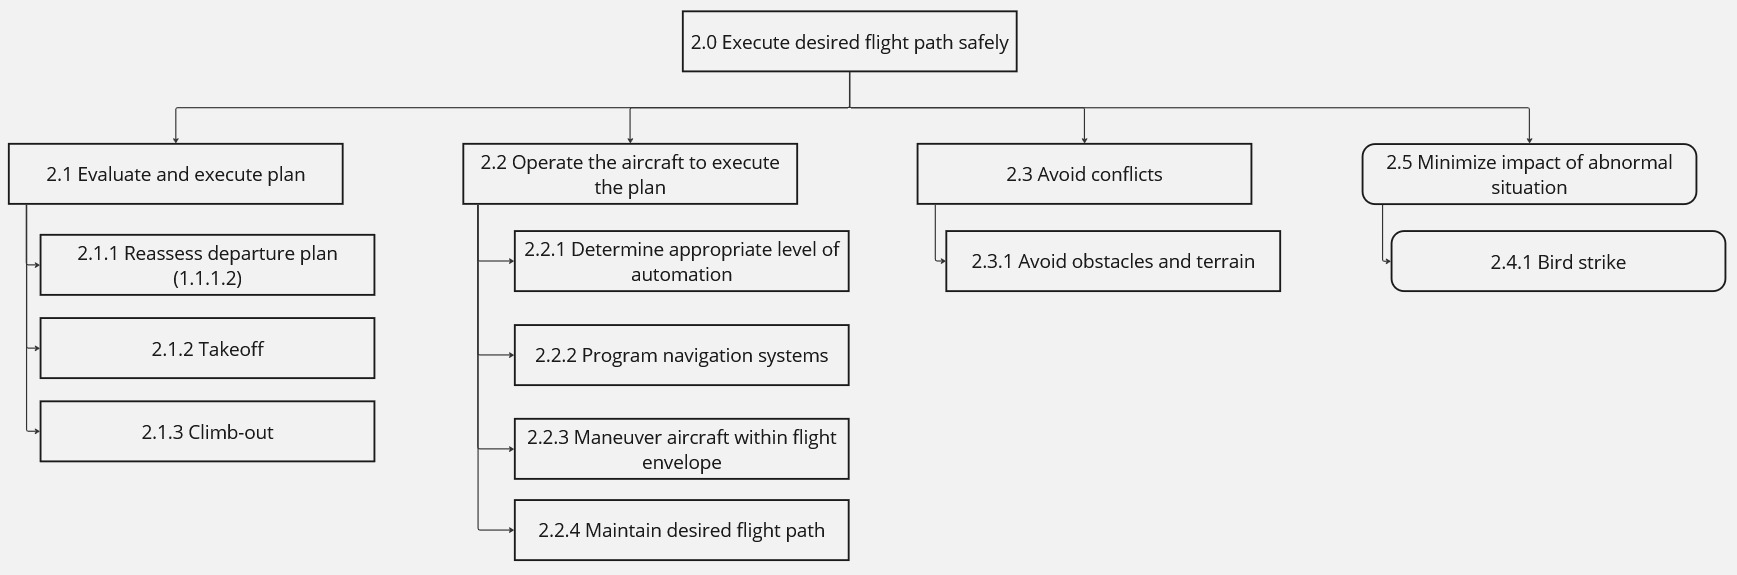
\includegraphics[width=1.0\textwidth]{./images/GDTA/top-goal-2.jpg}
		\label{gdta:top-2}
	\end{figure}

	\begin{figure}[H]
		\centering
		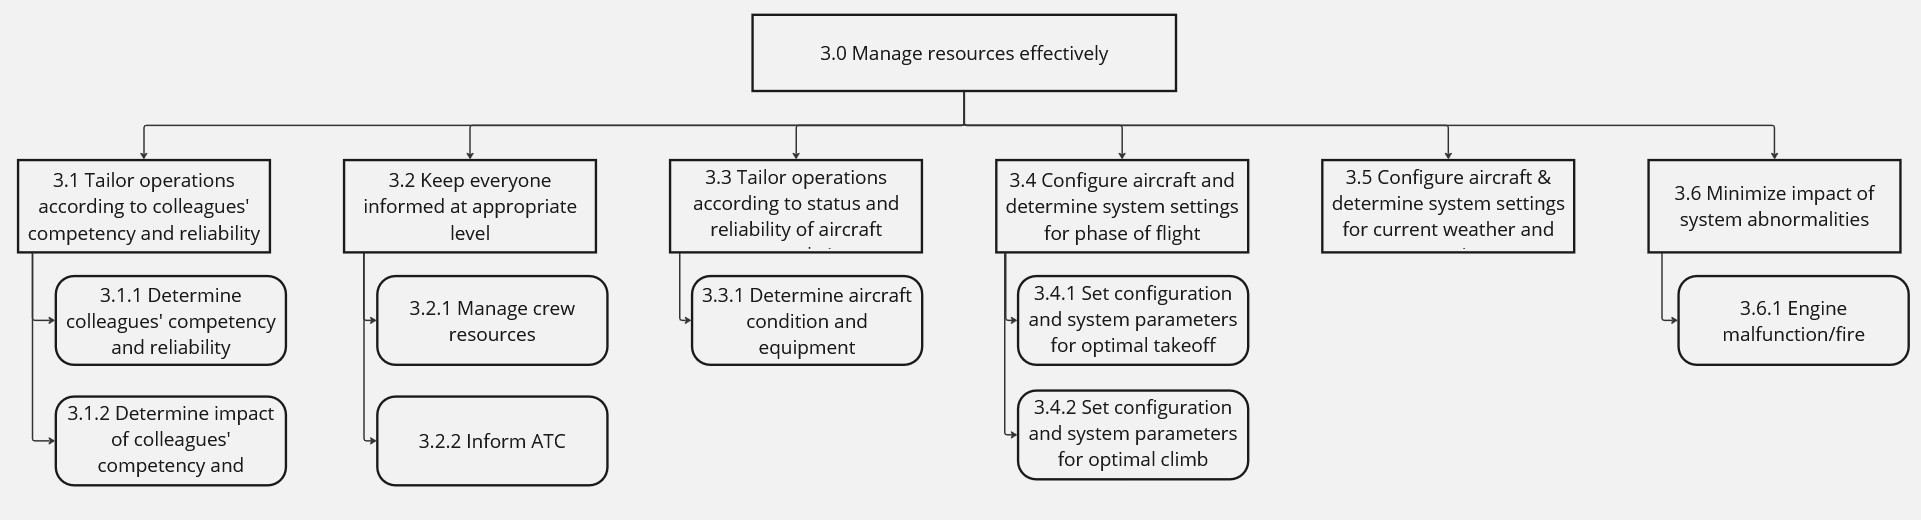
\includegraphics[width=1.0\textwidth]{./images/GDTA/top-goal-3.jpg}
		\label{gdta:top-3}
	\end{figure}

	\subsection{Low-Level Goal hierarchy, SA questions and information requirements}

	\begin{figure}[H]
		\centering
		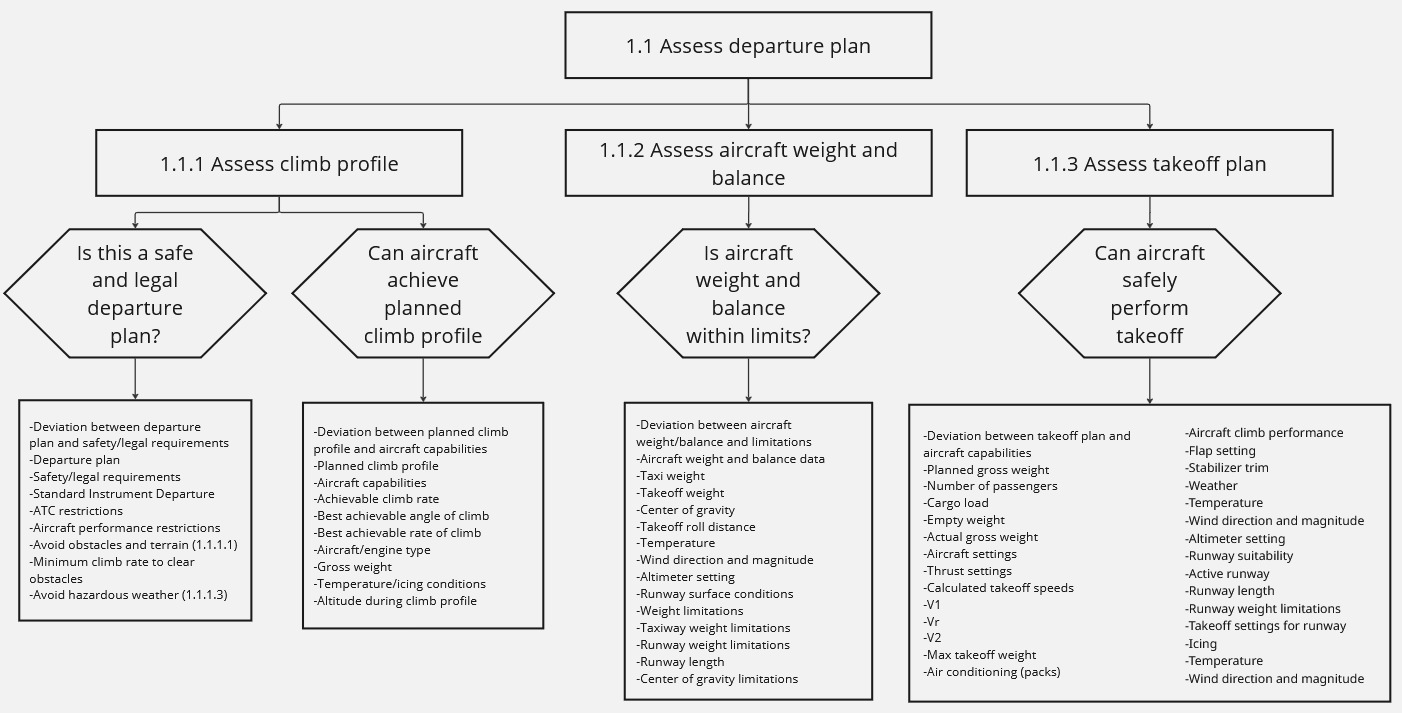
\includegraphics[width=1.0\textwidth]{./images/GDTA/bott-goal-1.jpg}
		\label{gdta:bott-1}
	\end{figure}

	\begin{figure}[H]
		\centering
		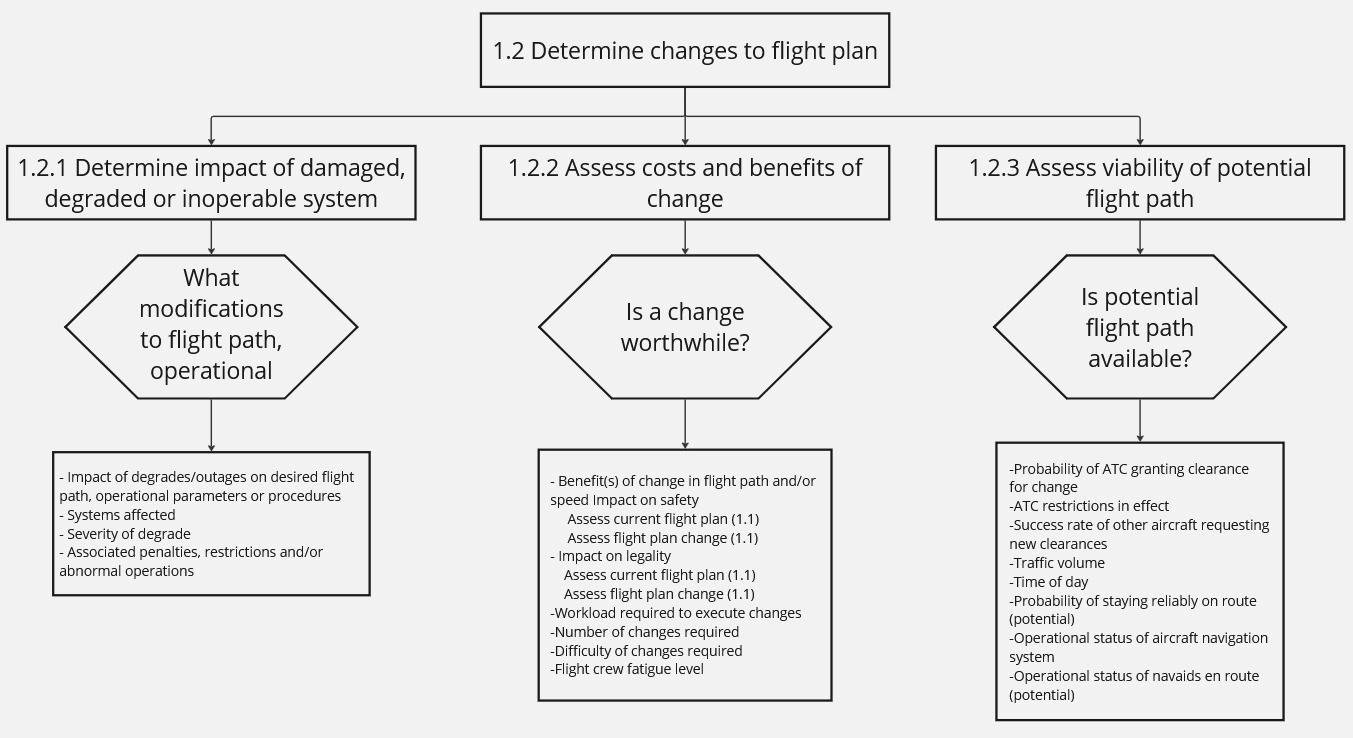
\includegraphics[width=1.0\textwidth]{./images/GDTA/bott-goal-2.jpg}
		\label{gdta:bott-2}
	\end{figure}

	\begin{figure}[H]
		\centering
		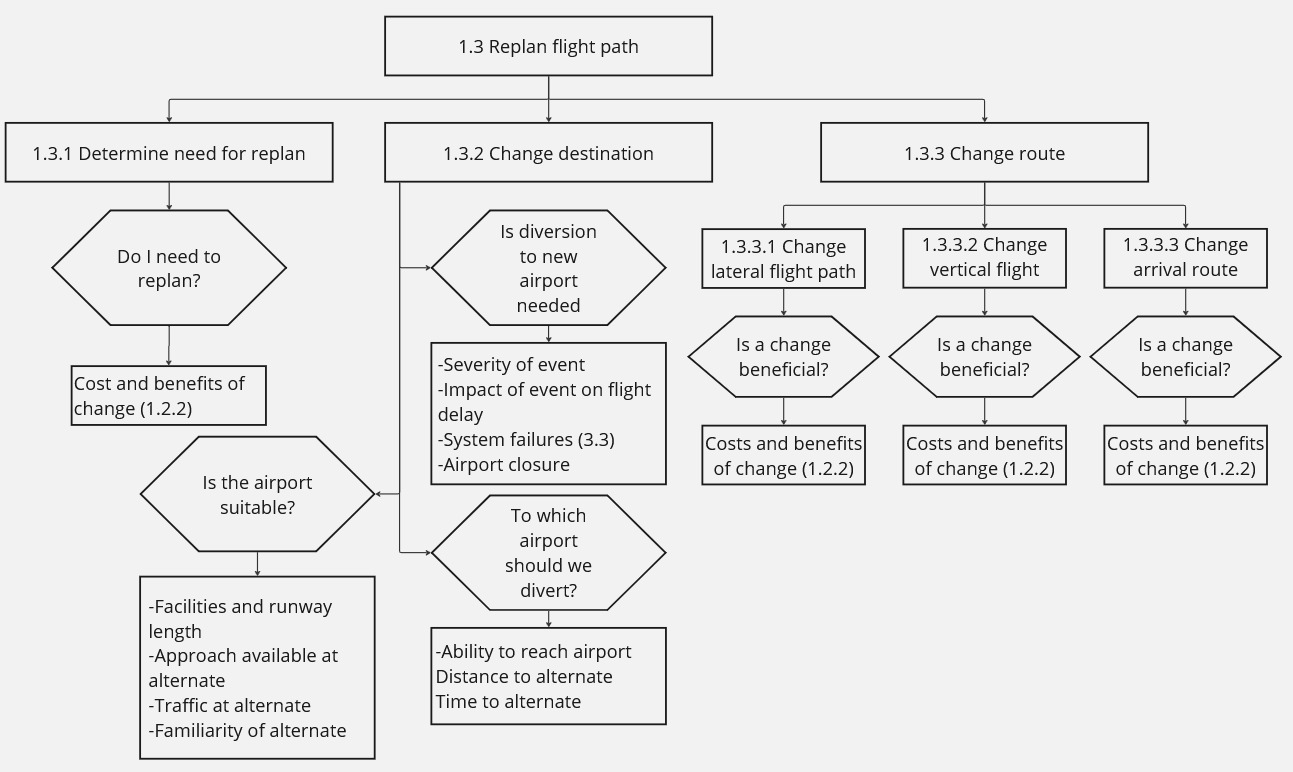
\includegraphics[width=1.0\textwidth]{./images/GDTA/bott-goal-3.jpg}
		\label{gdta:bott-3}
	\end{figure}

	\begin{figure}[H]
		\centering
		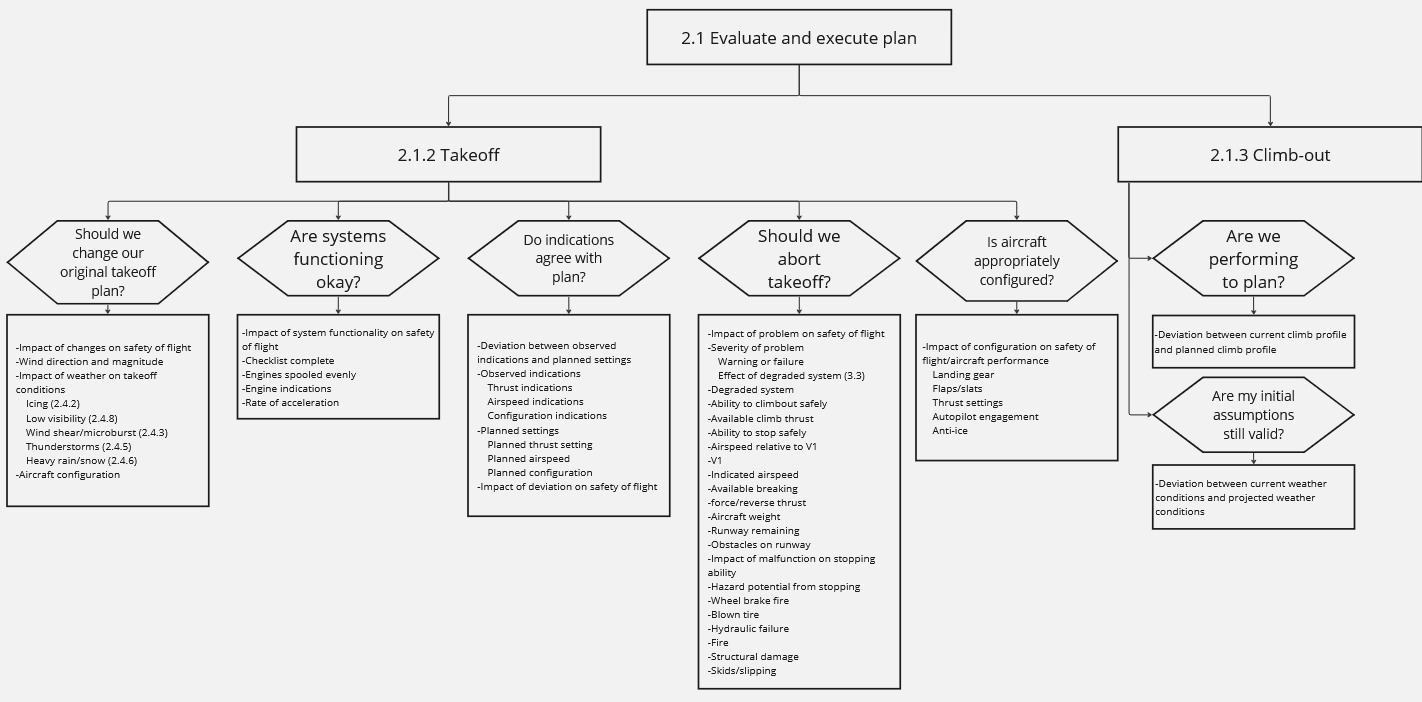
\includegraphics[width=1.0\textwidth]{./images/GDTA/bott-goal-4.jpg}
		\label{gdta:bott-4}
	\end{figure}

	\begin{figure}[H]
		\centering
		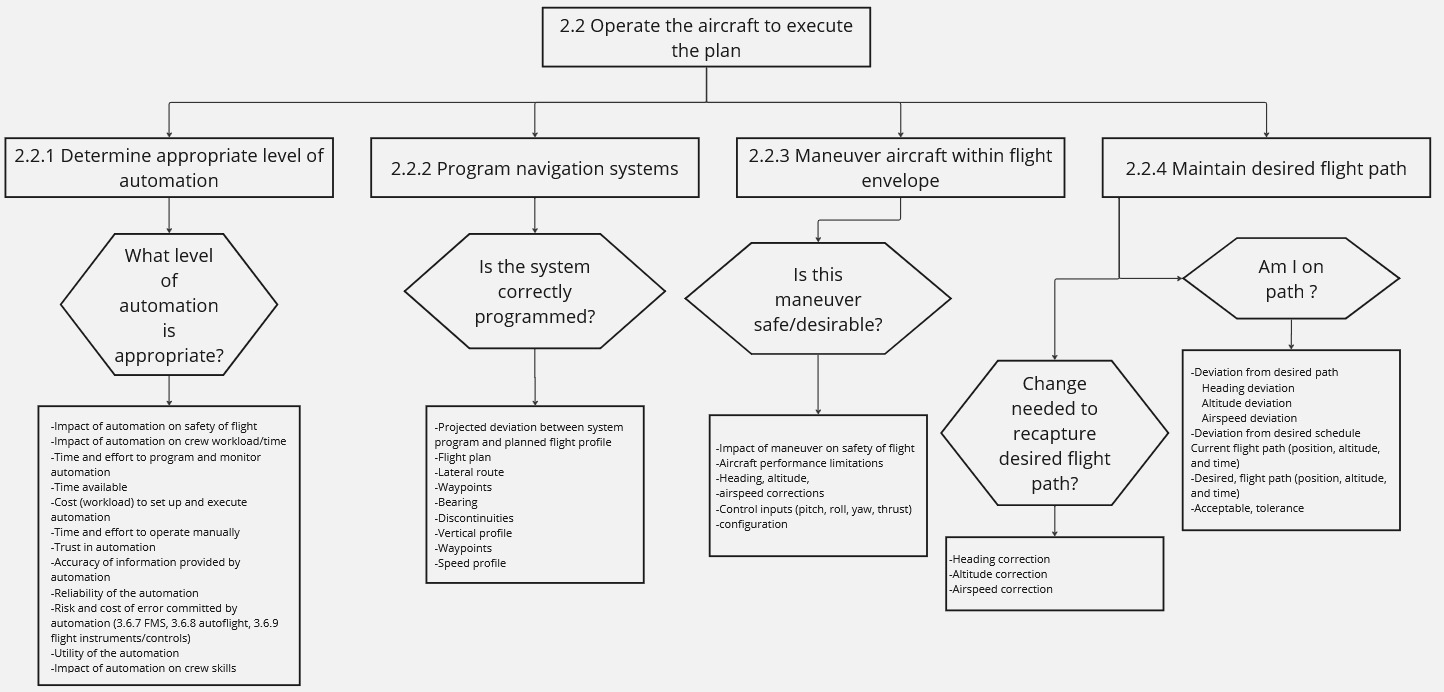
\includegraphics[width=1.0\textwidth]{./images/GDTA/bott-goal-5.jpg}
		\label{gdta:bott-5}
	\end{figure}

	\begin{figure}[H]
		\centering
		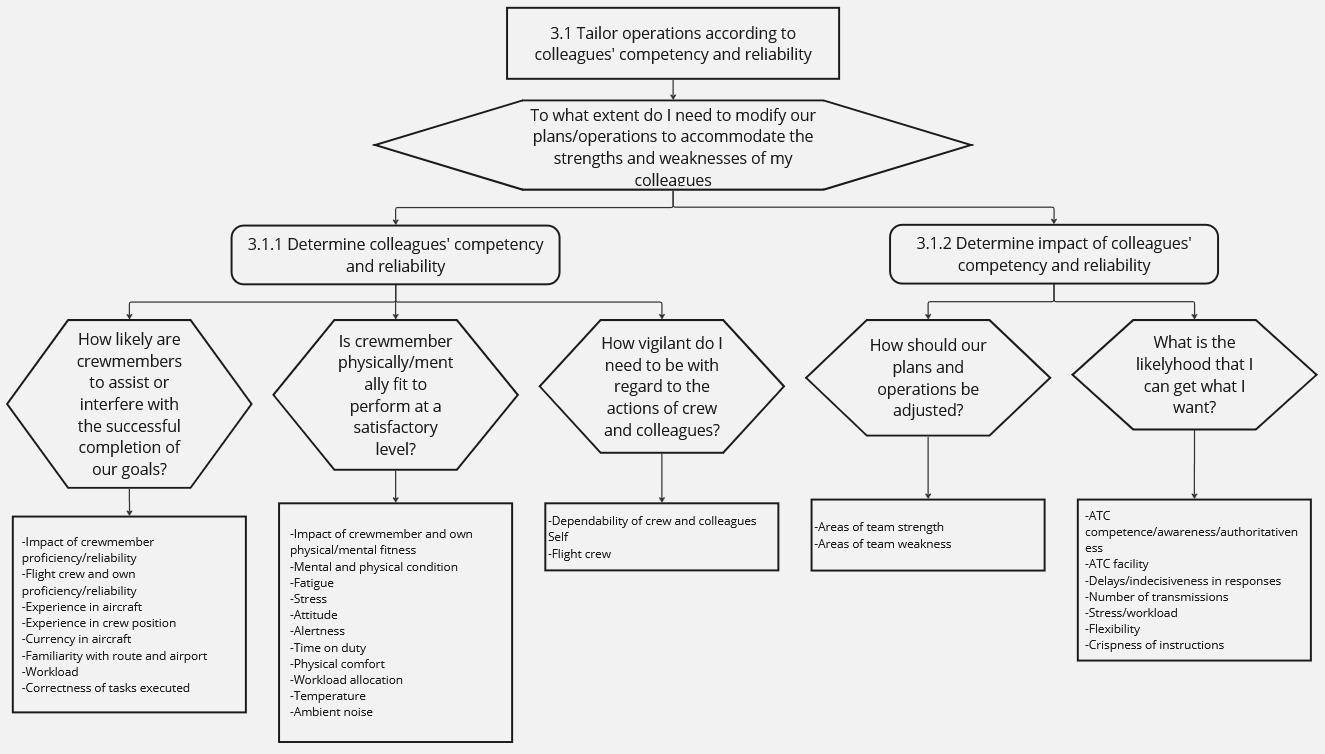
\includegraphics[width=1.0\textwidth]{./images/GDTA/bott-goal-6.jpg}
		\label{gdta:bott-6}
	\end{figure}

	\begin{figure}[H]
		\centering
		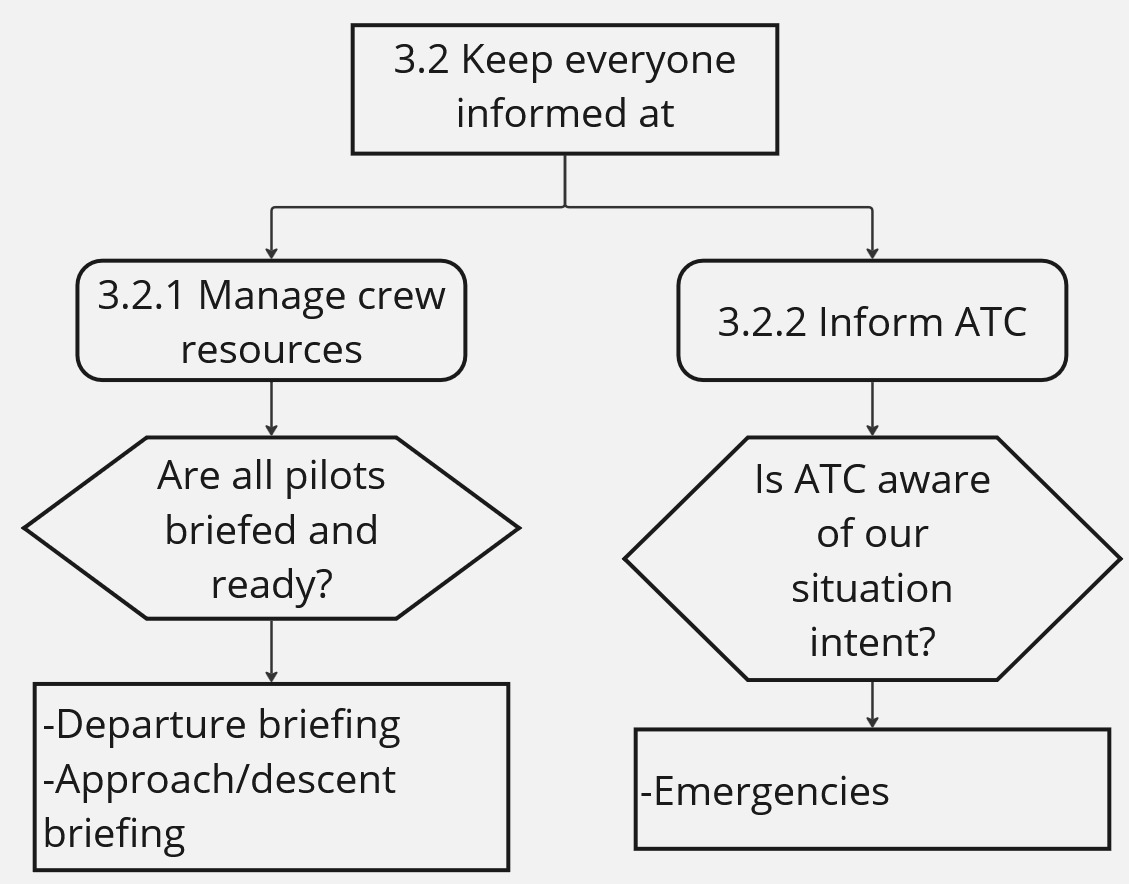
\includegraphics[width=0.8\textwidth]{./images/GDTA/bott-goal-7.jpg}
		\label{gdta:bott-7}
	\end{figure}

	\begin{figure}[H]
		\centering
		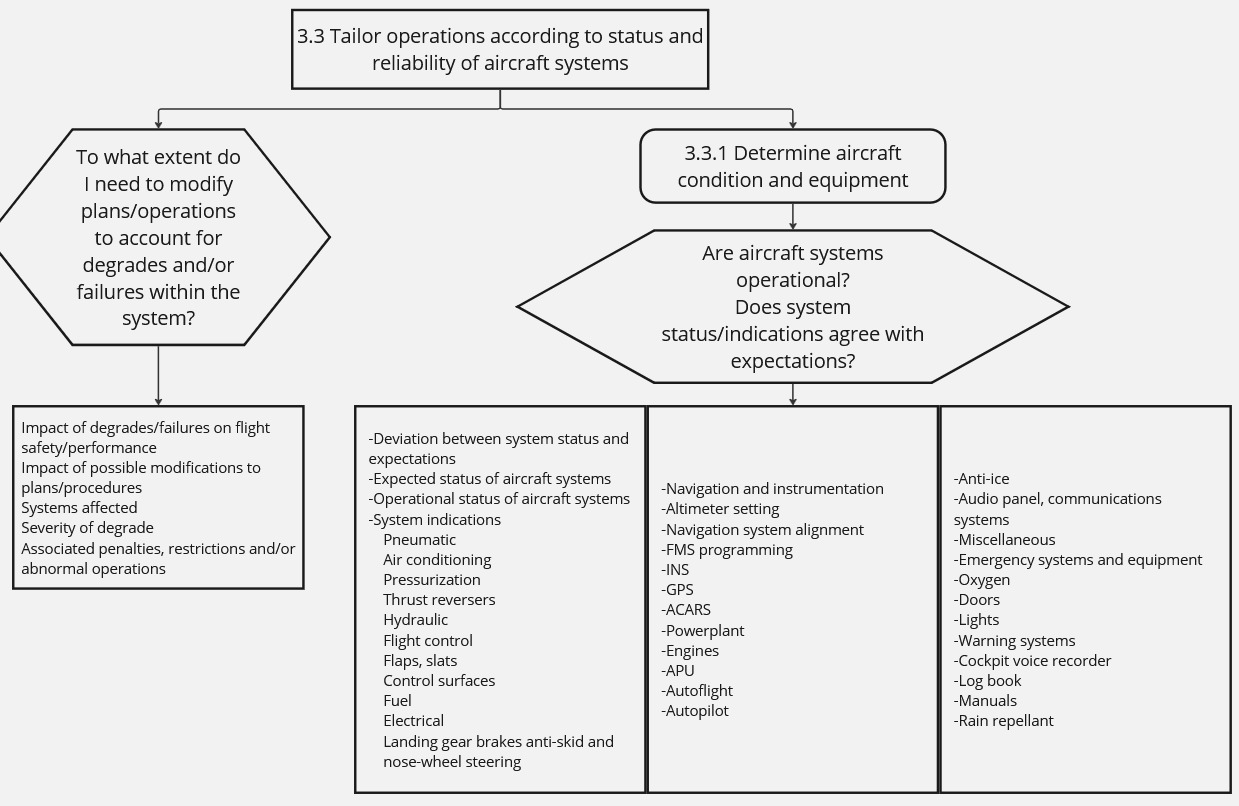
\includegraphics[width=1.0\textwidth]{./images/GDTA/bott-goal-8.jpg}
		\label{gdta:bott-8}
	\end{figure}

	\begin{figure}[H]
		\centering
		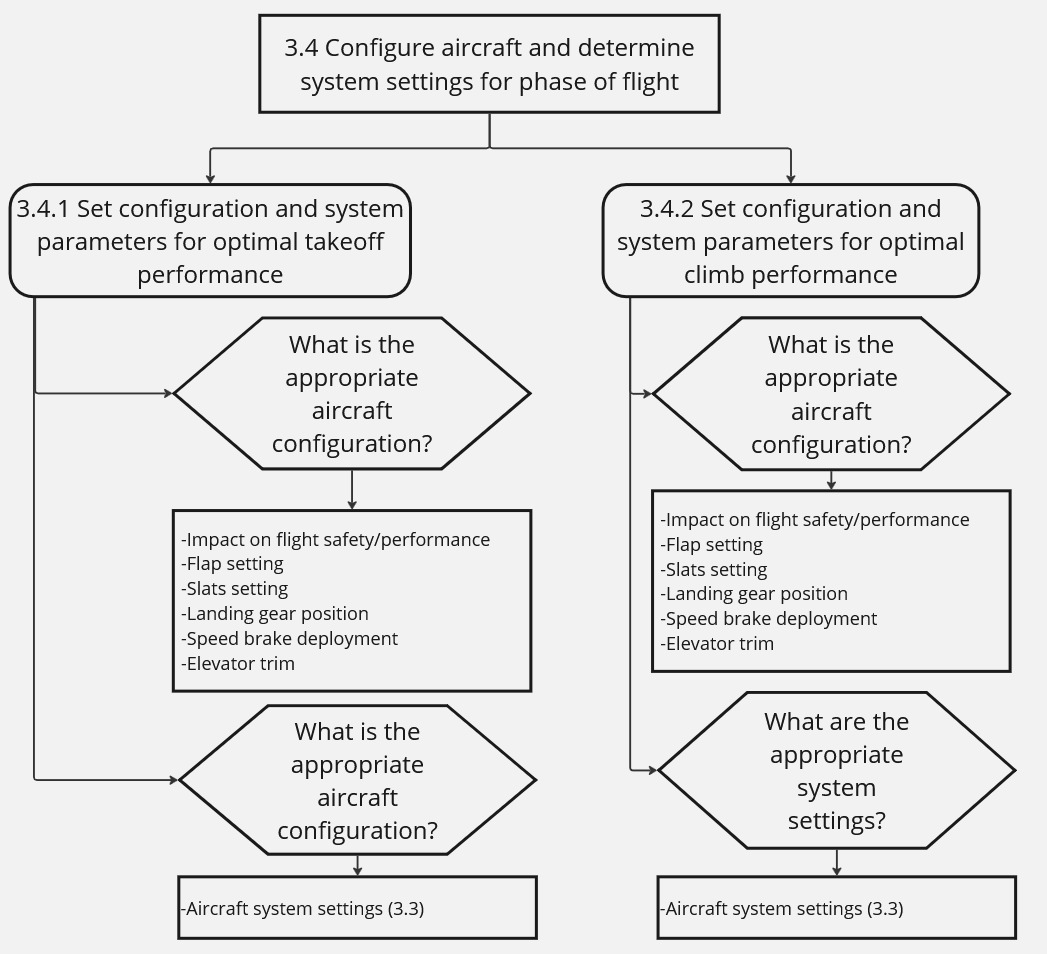
\includegraphics[width=0.8\textwidth]{./images/GDTA/bott-goal-9.jpg}
		\label{gdta:bott-9}
	\end{figure}

	\begin{figure}[H]
		\centering
		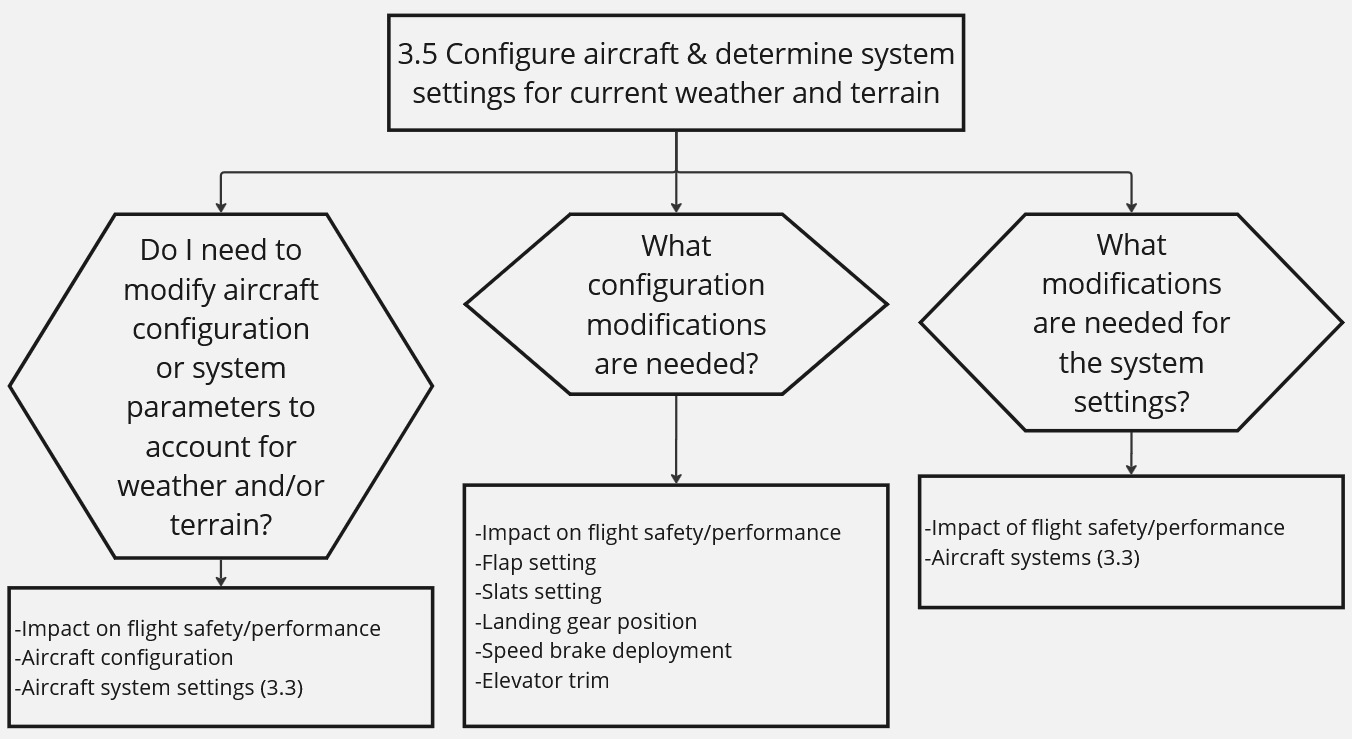
\includegraphics[width=1.0\textwidth]{./images/GDTA/bott-goal-10.jpg}
		\label{gdta:bott-10}
	\end{figure}

	\begin{figure}[H]
		\centering
		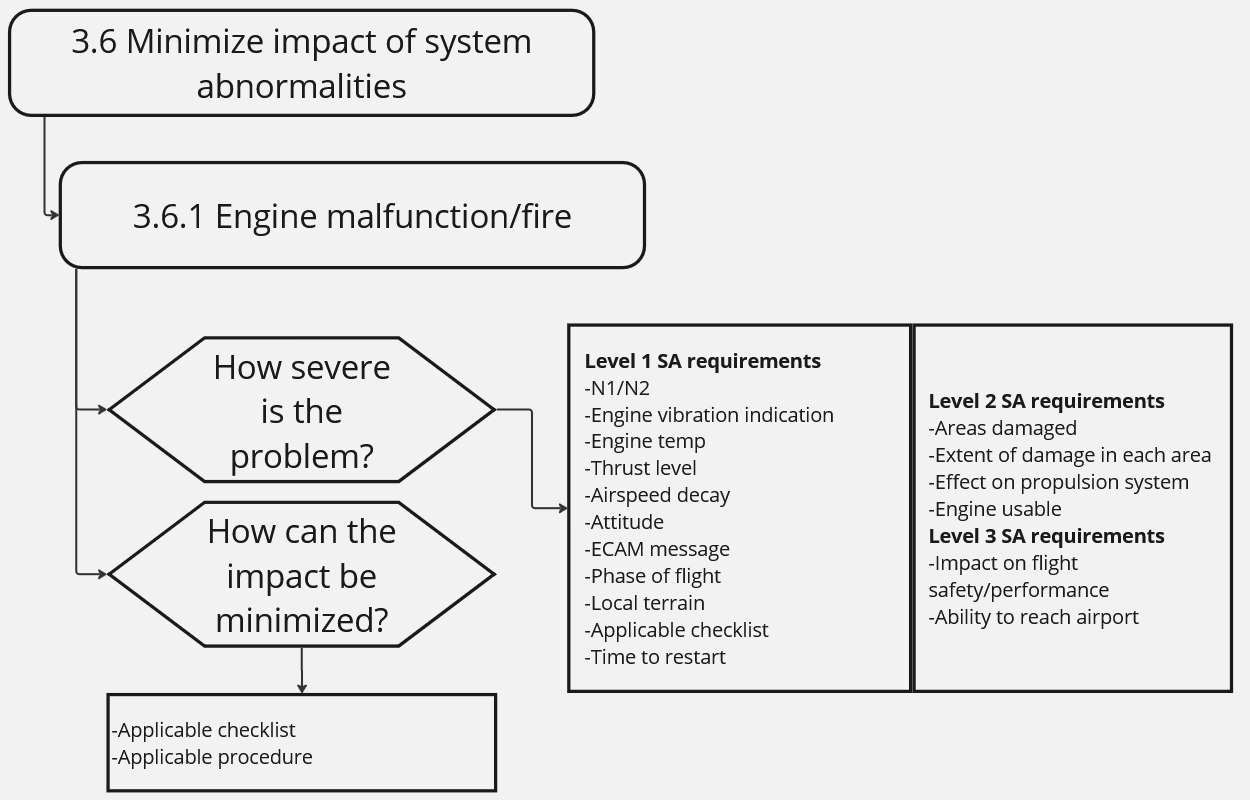
\includegraphics[width=1.0\textwidth]{./images/GDTA/bott-goal-11.jpg}
		\label{gdta:bott-11}
	\end{figure}

	\section{Interdependence Analysis}
	\label{appendix:IA}

	\subsection{Color key for Interdependence Analysis}

	\begin{table}[H]
		\centering
		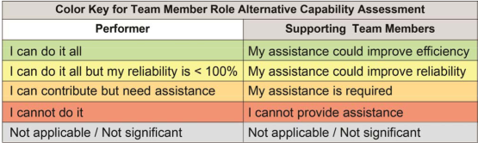
\includegraphics{images/color_key_IA.png}
		\label{table:color-key}
	\end{table}

	\subsection{IA tables}
	\label{table:all-IA}

	\begin{table}[H]
		\centering
		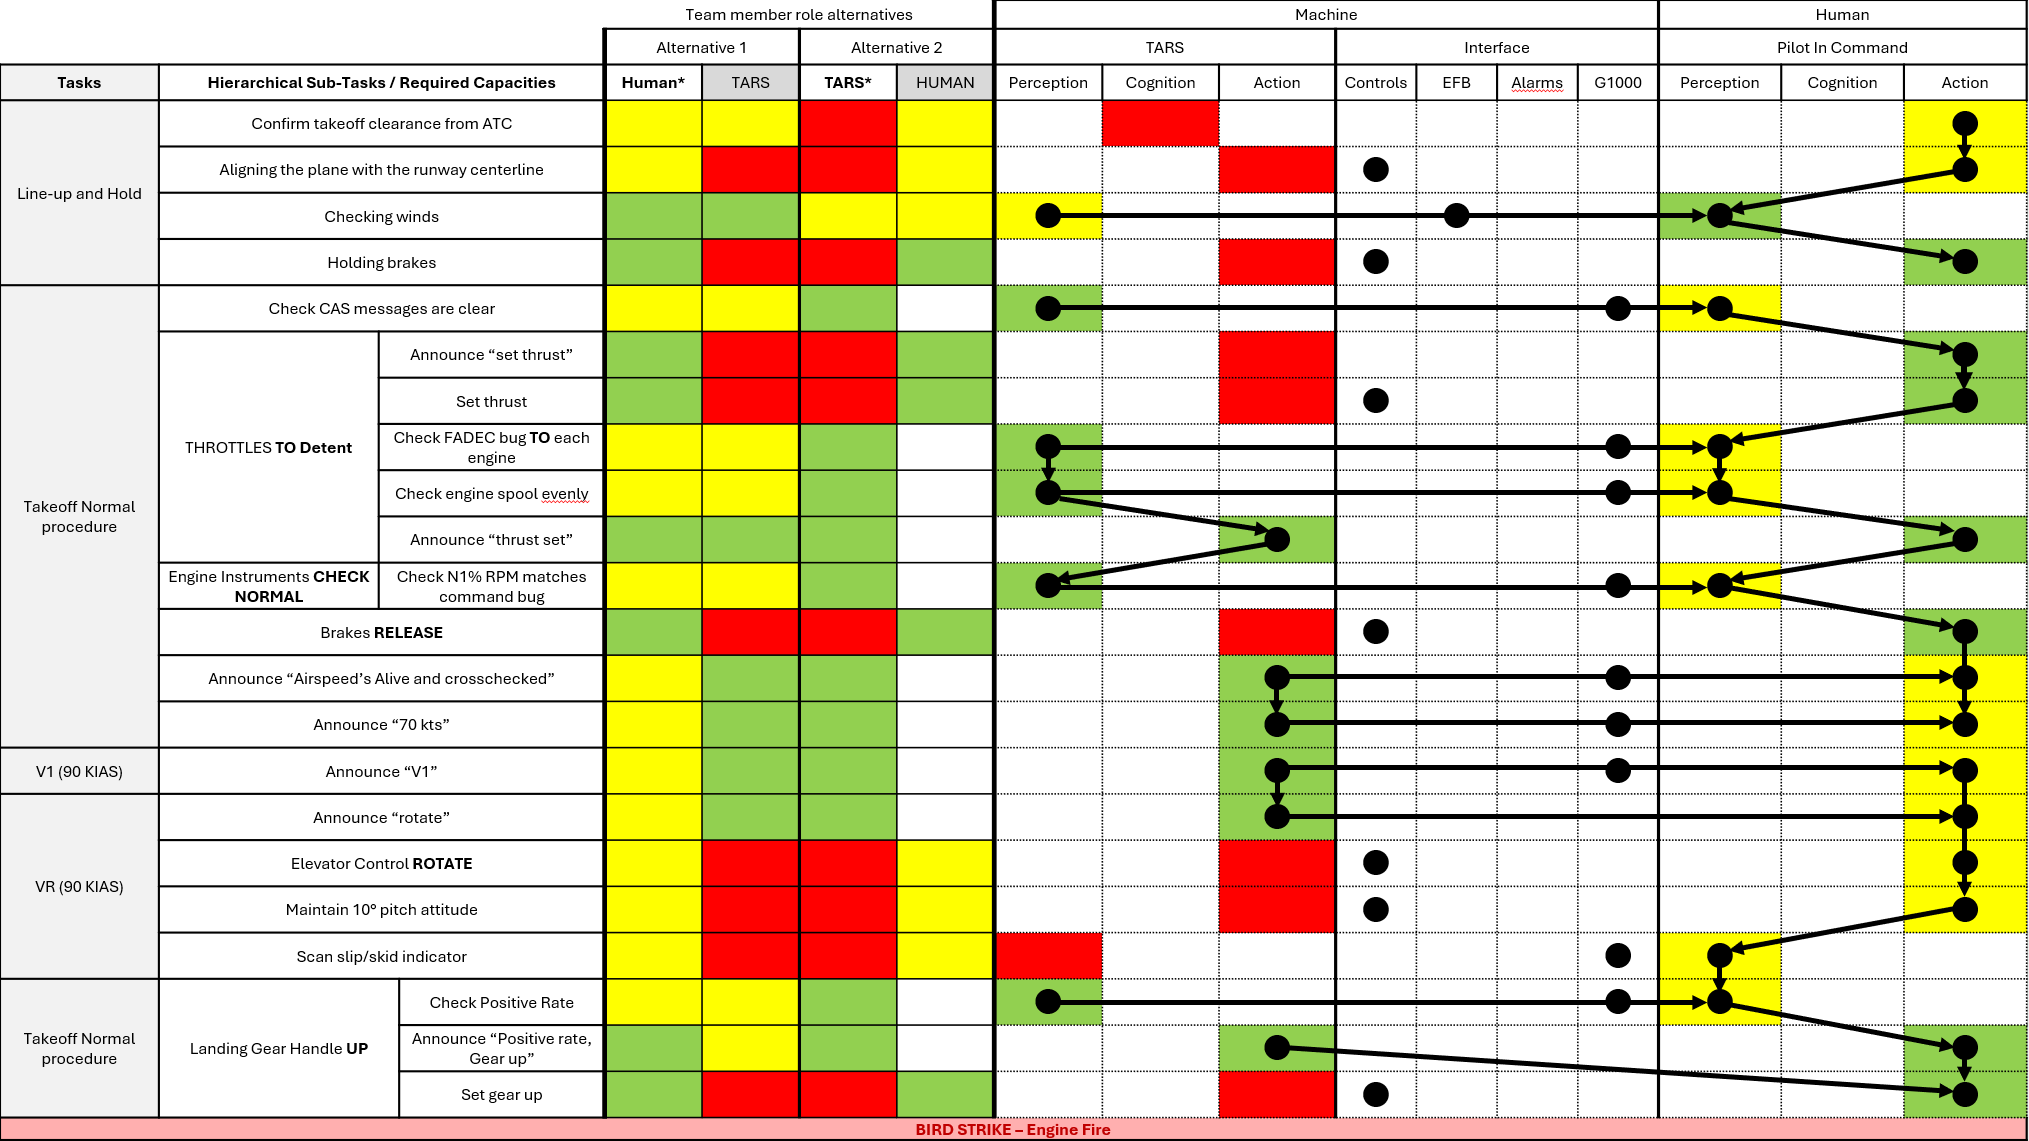
\includegraphics[width=1\textwidth]{images/IA-table-1.png}
	\end{table}

	\begin{table}[H]
		\centering
		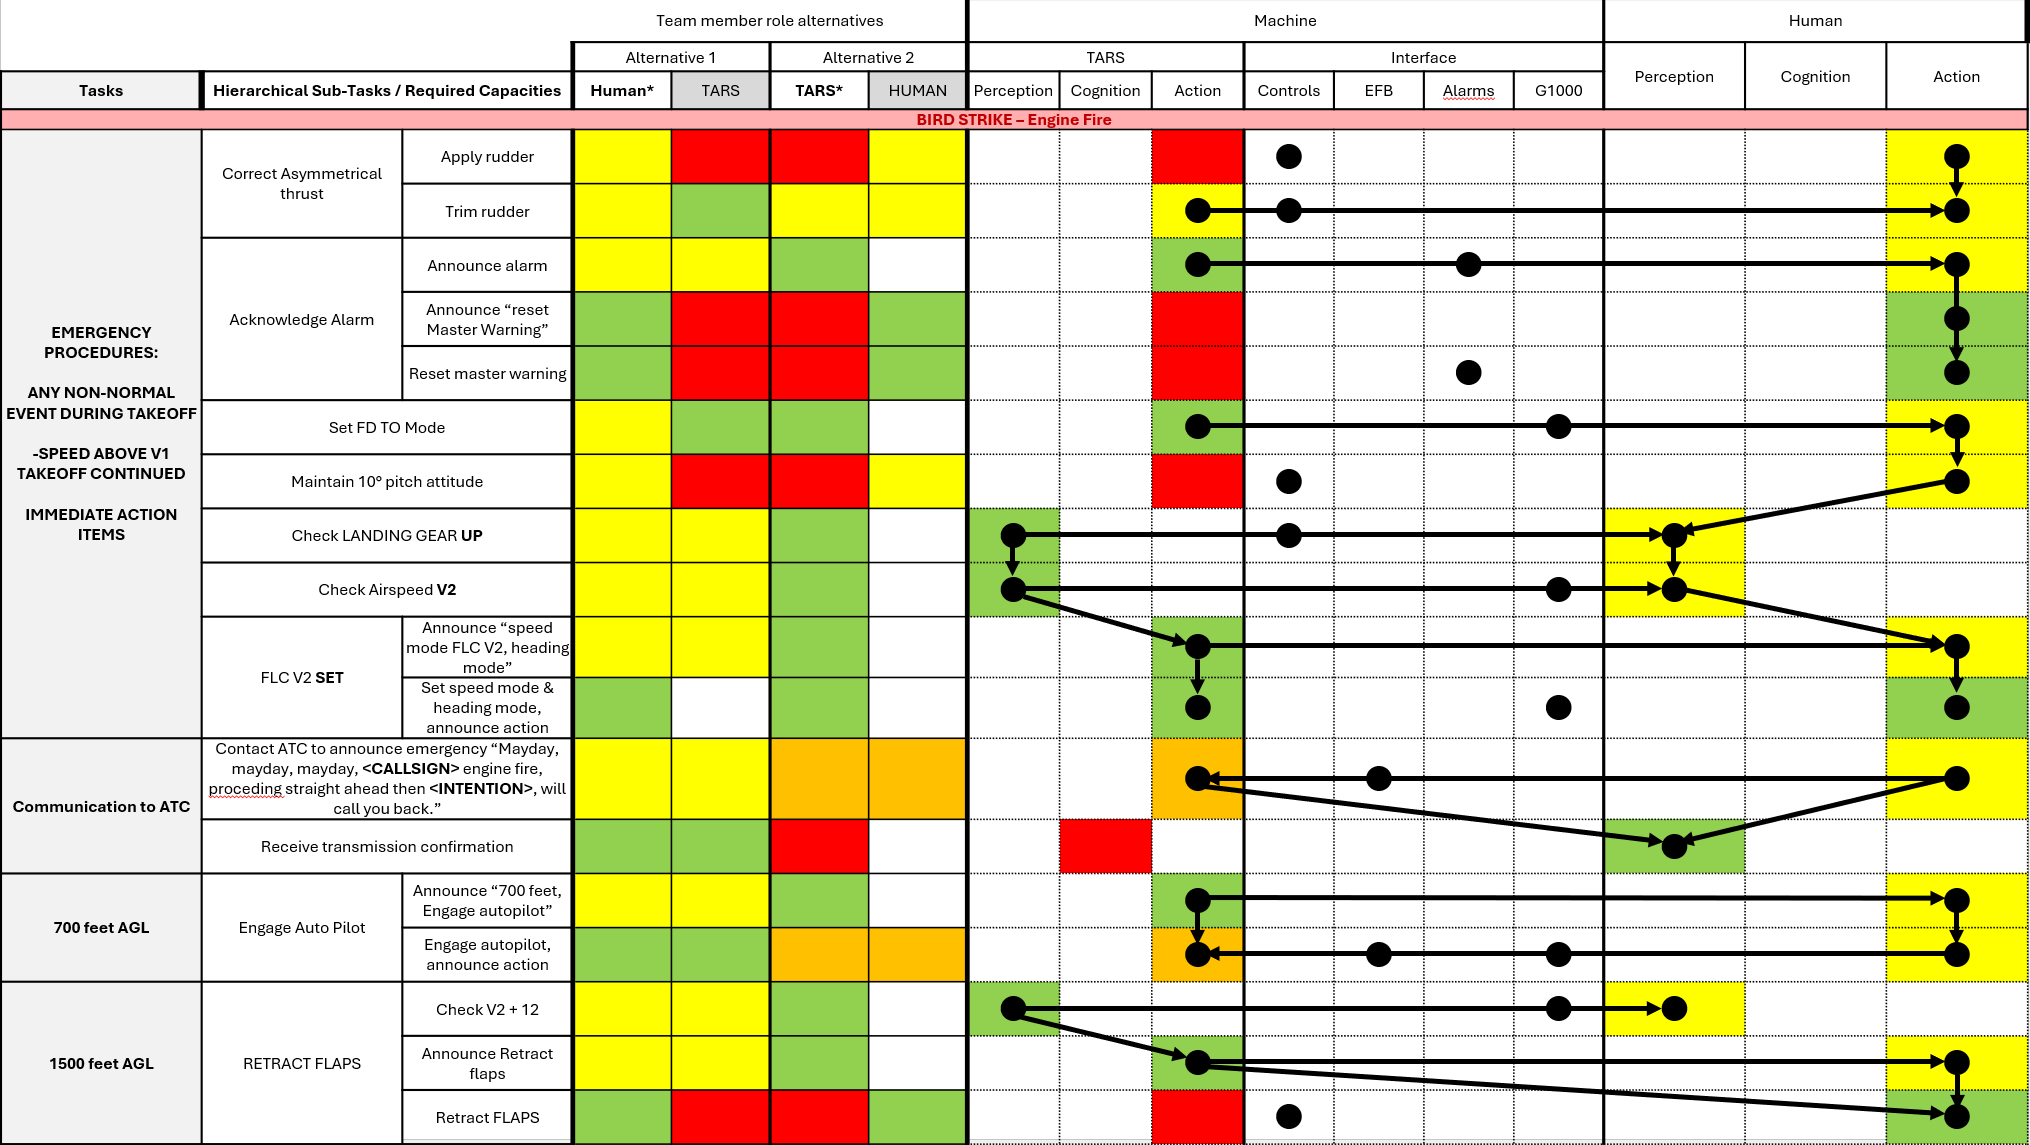
\includegraphics[width=1\textwidth]{images/IA-table-2.png}
	\end{table}

	\begin{table}[H]
		\centering
		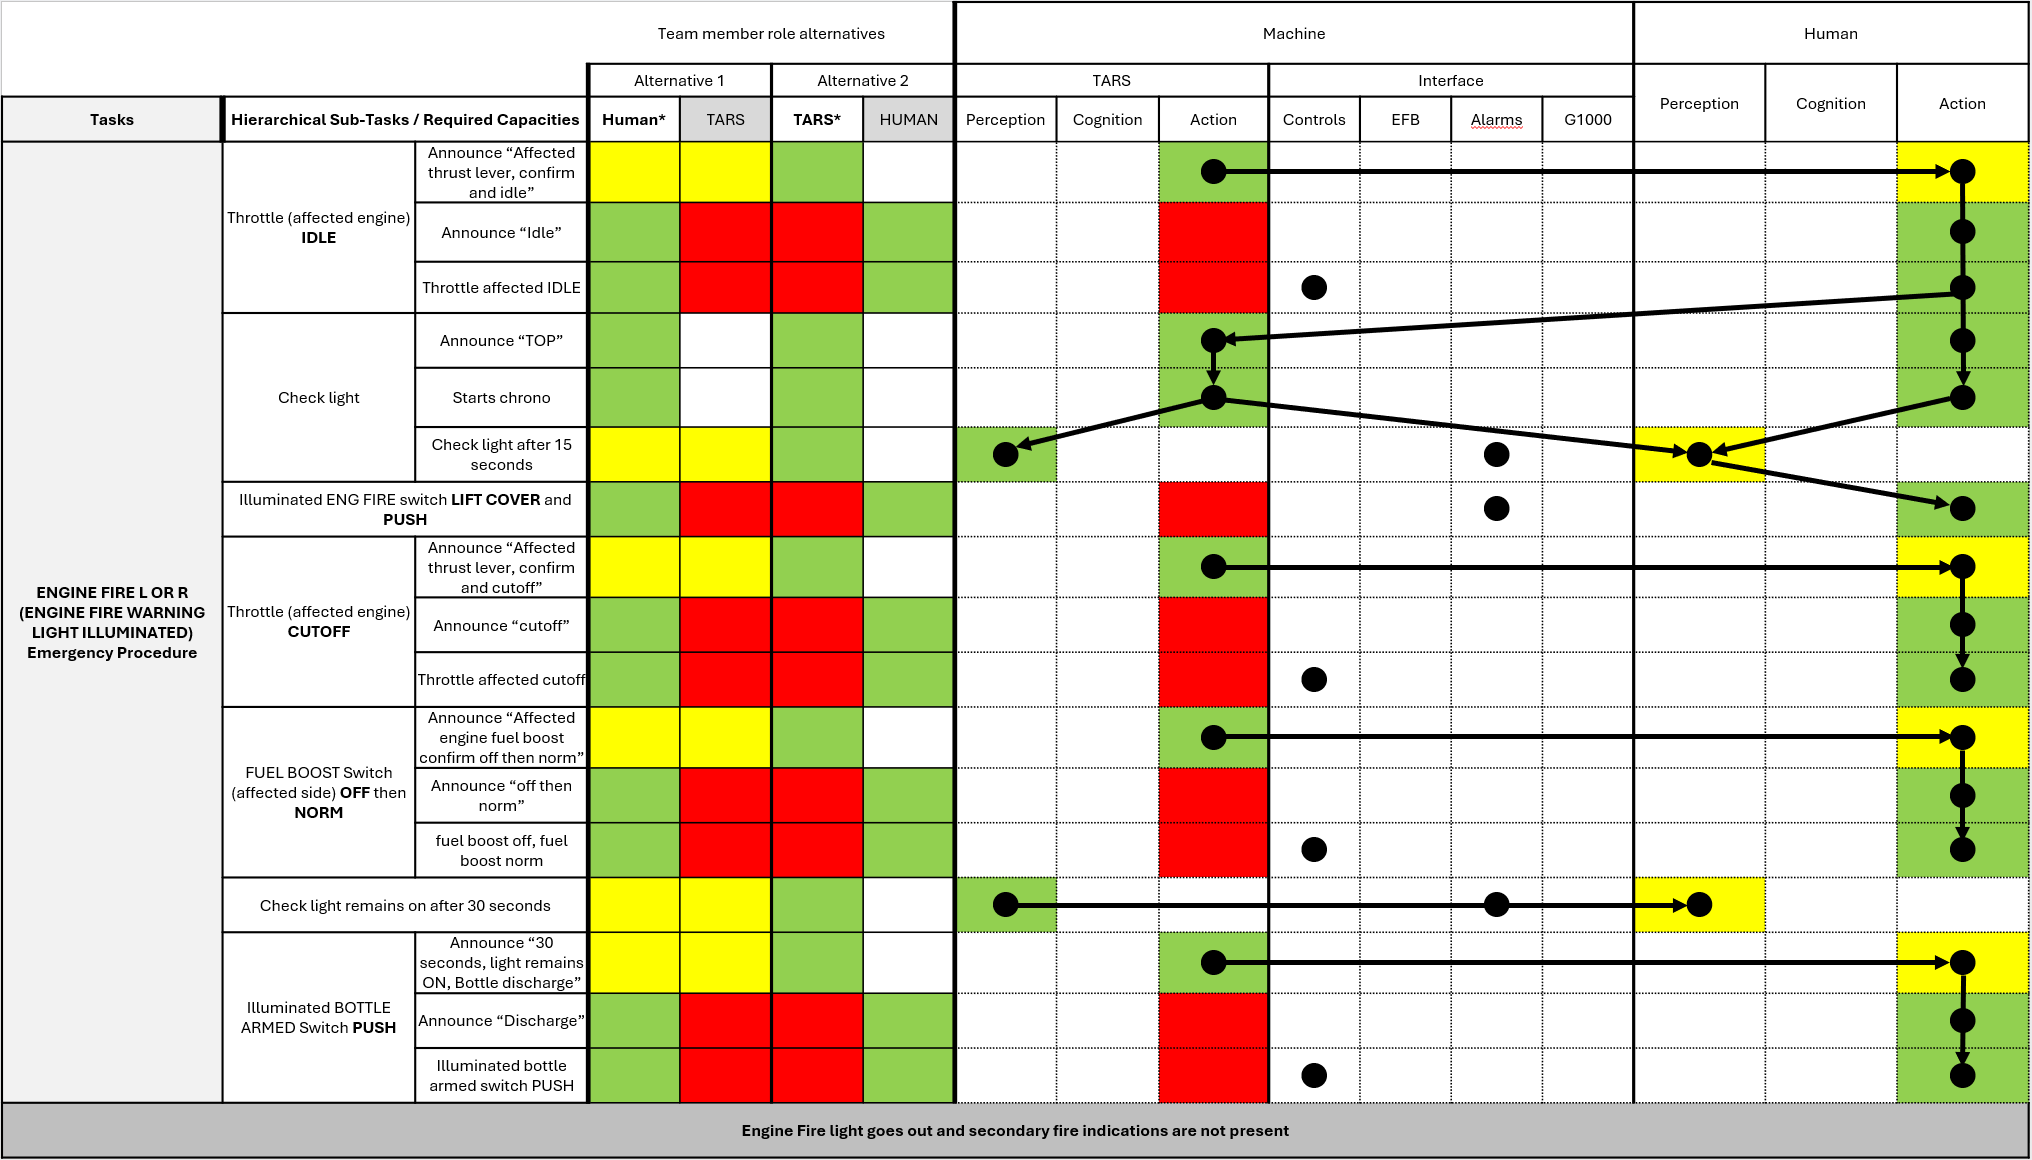
\includegraphics[width=1\textwidth]{images/IA-table-3.png}
	\end{table}

	\begin{table}[H]
		\centering
		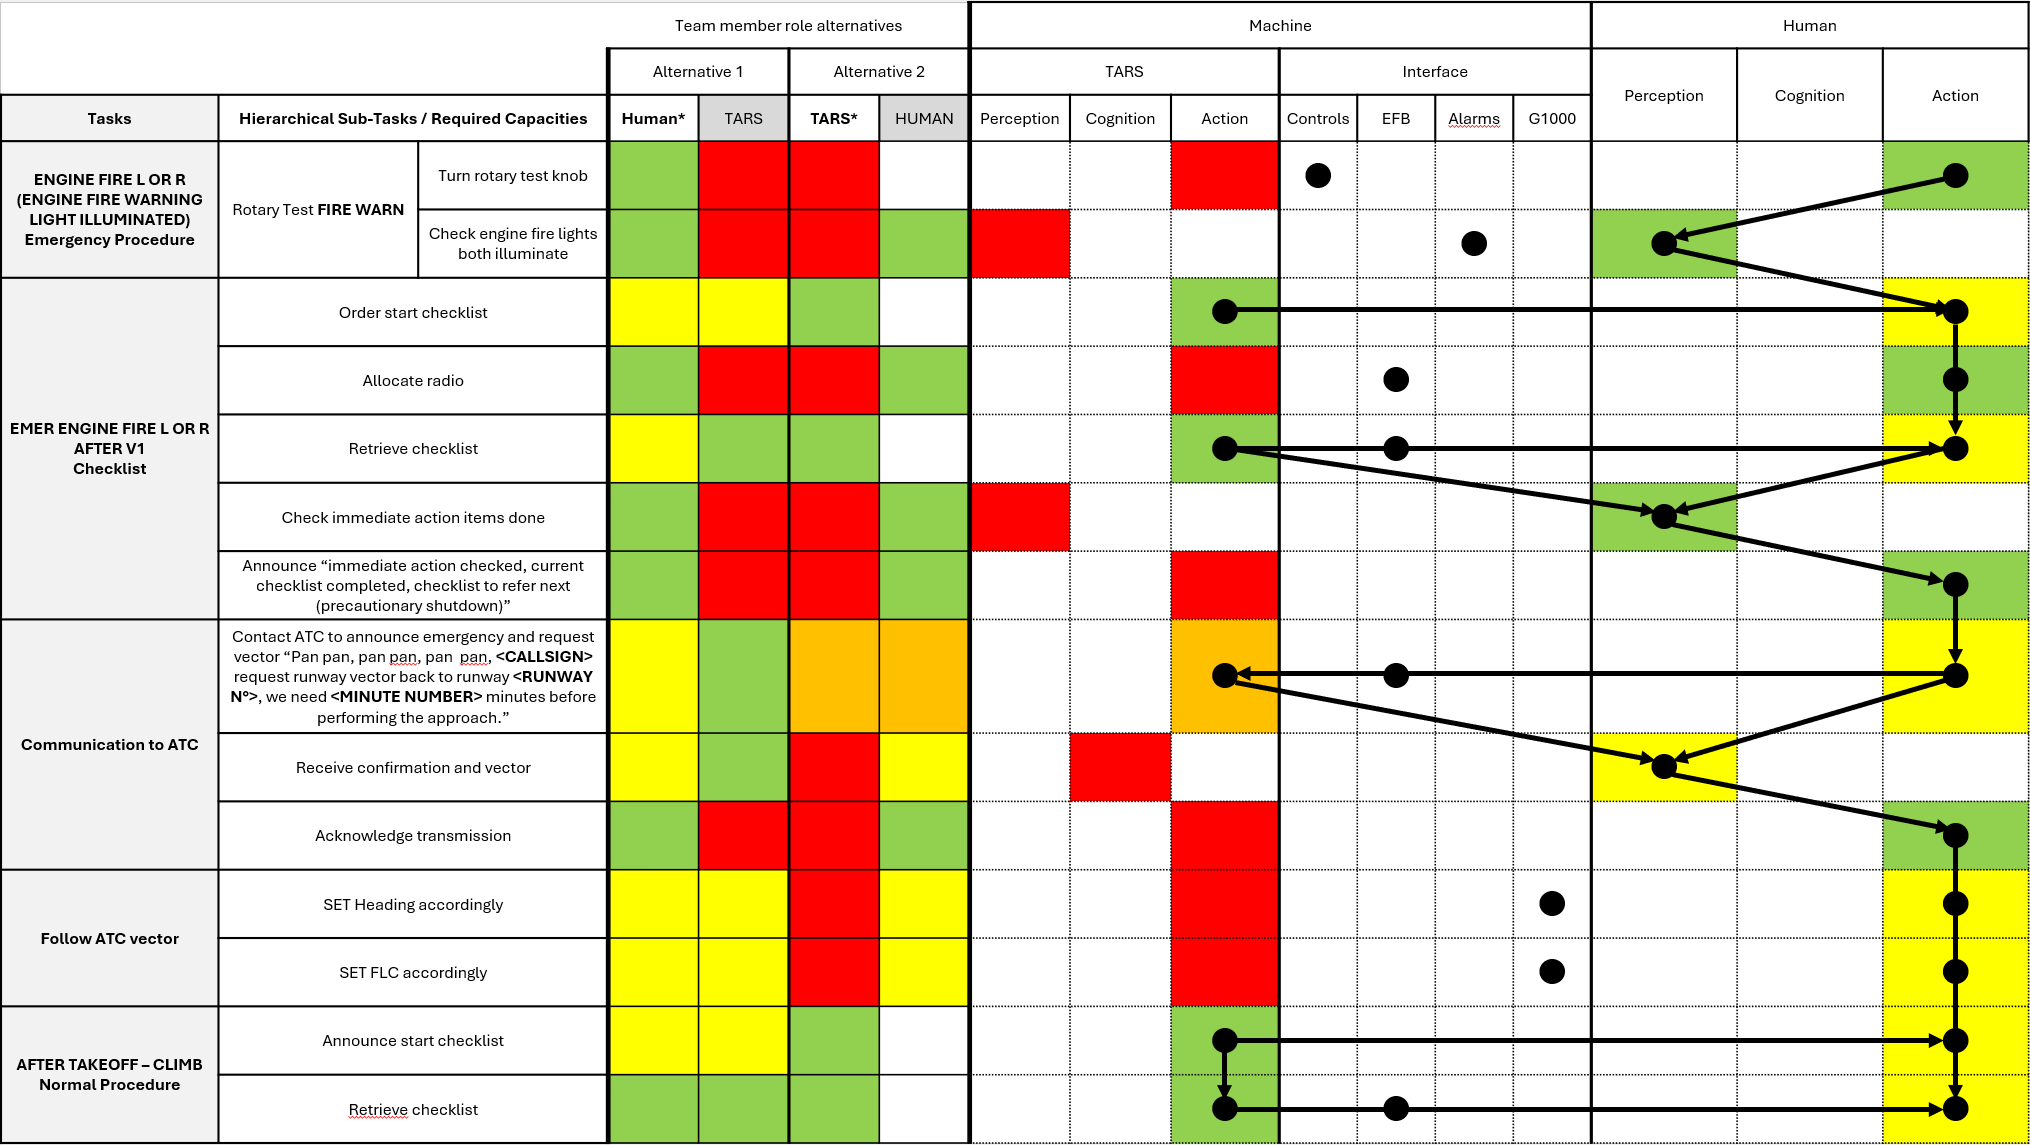
\includegraphics[width=1\textwidth]{images/IA-table-4.png}
	\end{table}

	\begin{table}[H]
		\centering
		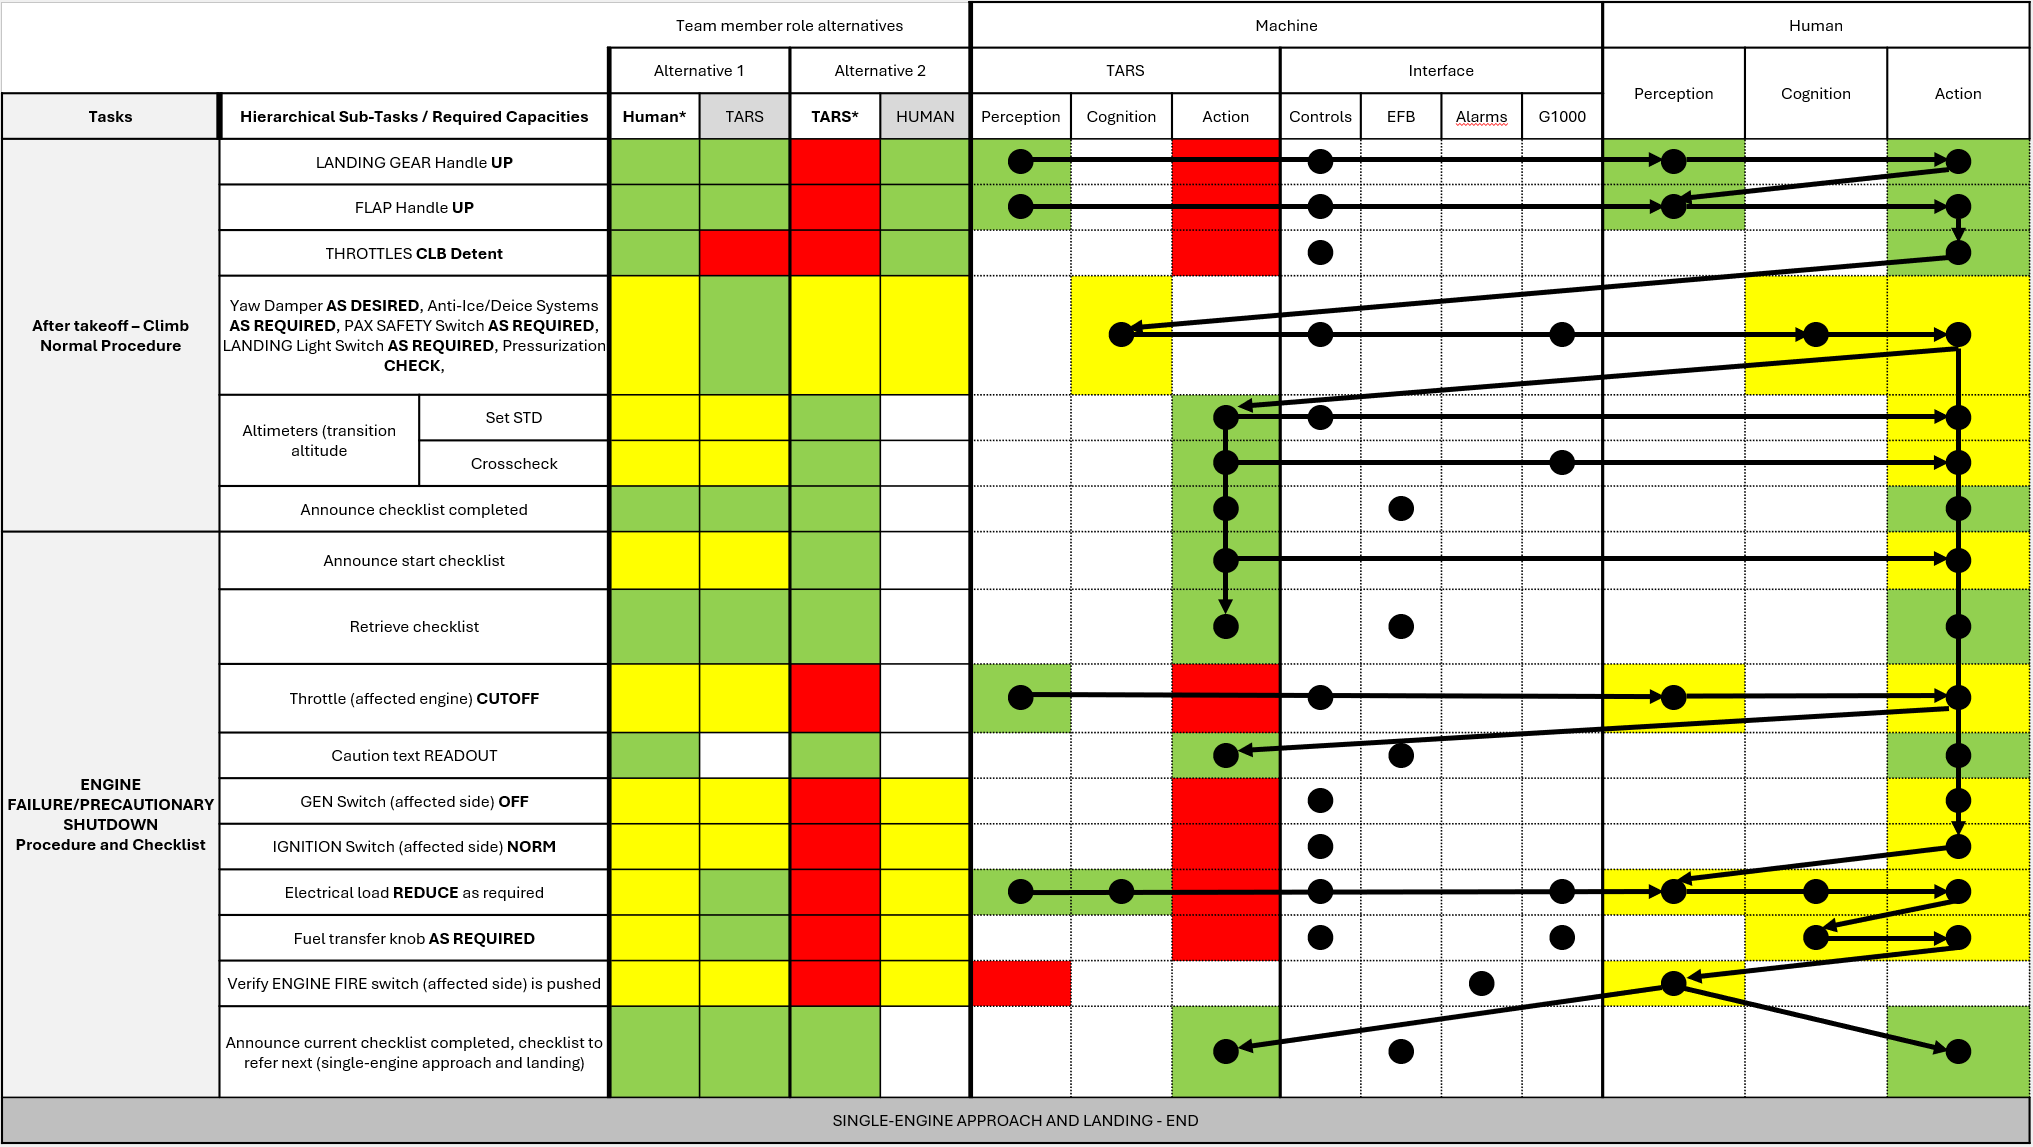
\includegraphics[width=1\textwidth]{images/IA-table-5.png}
	\end{table}

	\printbibliography % Prints the bibliography
\end{document} % Ends the document